\chapter{Results}    
\label{Ch:results}

\section{Tracking endocytic proteins in yeast}
\mbox{}\\
Sla1 is a late-stage endocytic coat protein. Since the coat moves inwards with the membrane as it invaginates, it serves as a marker for membrane invagination. Sla1 is used throughout this work to track coat movement. In Fig.3.1B, a kymograph of a Sla1-GFP patch at the plasma membrane of a yeast cell shows it arrives at endocytic sites, and after about 15 seconds, moves inwards into the cytoplasm. Actin-binding protein Abp1, which marks the actin network, also shows movement inwards almost as soon as it arrives at endocytic sites. Rvs167, the scission-stage protein, has a relatively short lifetime, and shows a sharp jump into the cytoplasm. 


\vspace{7mm}
Averaged centroid tracking in live cells, as described in Picco et al. 1, can quantify this movement and dynamics of endocytic. Briefly described, yeast cells expressing fluorescently-tagged endocytic proteins are imaged at the equatorial plane. Since membrane invagination progresses perpendicularly to the plane of the plasma membrane, proteins patches that move inward with membrane invagination do so in the imaging plane. Centroids of a particular protein as it forms patches at endocytic sites are thus tracked in time. Between 40-50 centroids of each protein are averaged. This provides an averaged centroid that can be followed with high spatial and temporal resolution. When different endocytic proteins are simultaneously imaged with the abundant Abp1, Abp1 provides a frame of reference to which all the proteins can be aligned. Averaged centroid tracking, and correlating these centroid movements with membrane shapes acquired by correlative light and electron microscopy (CLEM) allows us to understand the dynamics of these proteins in the context of shape transitions of the membrane1.  


\vspace{7mm}
Correlating CLEM and centroid tracking has shown that Sla1 starts to moves into the cytoplasm concomitant with the arrival of Abp1, and therefore of actin1–3. Sla1 moves inwards along with the membrane and follows it through endocytosis. As inward movement of the coat begins, the Sla1 patch is disassembled, inferred from the decay of the fluorescent intensity of Sla1-GFP1 (Fig.3.1D,E). Rvs localizes to endocytic patches later in the endocytic timeline, after parallel membrane tubes are formed3. Membrane scission occurs at around 60\% of its lifetime at sites3. At the time of scission, the Rvs167-GFP centroid shows a sharp jump into the cytoplasm, while fluorescent intensity shows a sudden decay, a profile that is unique among endocytic proteins1,3. Rvs is proposed to form a scaffold at the membrane tube. At scission time, this scaffold is thought to disassemble, resulting in an inward jump of the Rvs167 centroid to protein localized at the base of the newly formed vesicle. Abp1 intensity peaks at scission time, and consequently drops, indicating disassembly of the actin network upon vesicle formation. At scission time, the Sla1 centroid has moved about 140nm into the cytoplasm. Sla1 centroid can be tracked about 2-3 seconds after scission occurs. This portion of the centroid movement is marked by an increase in noise in fluorescent signal, and corresponds to diffusion of the vesicle after scission.


\vspace{7mm}
Averaged centroid tracking as in Picco et al., is used throughout this work to quantify the movement of endocytic proteins. Averaged centroid movement is referred to as “movement”. Unless indicated otherwise, “scission time” in all the centroid movement plots refers to the fluorescent intensity maximum of averaged Abp1 patches.

	\begin{figure}[H]
	\centering
	\hspace*{-1.8cm}%
	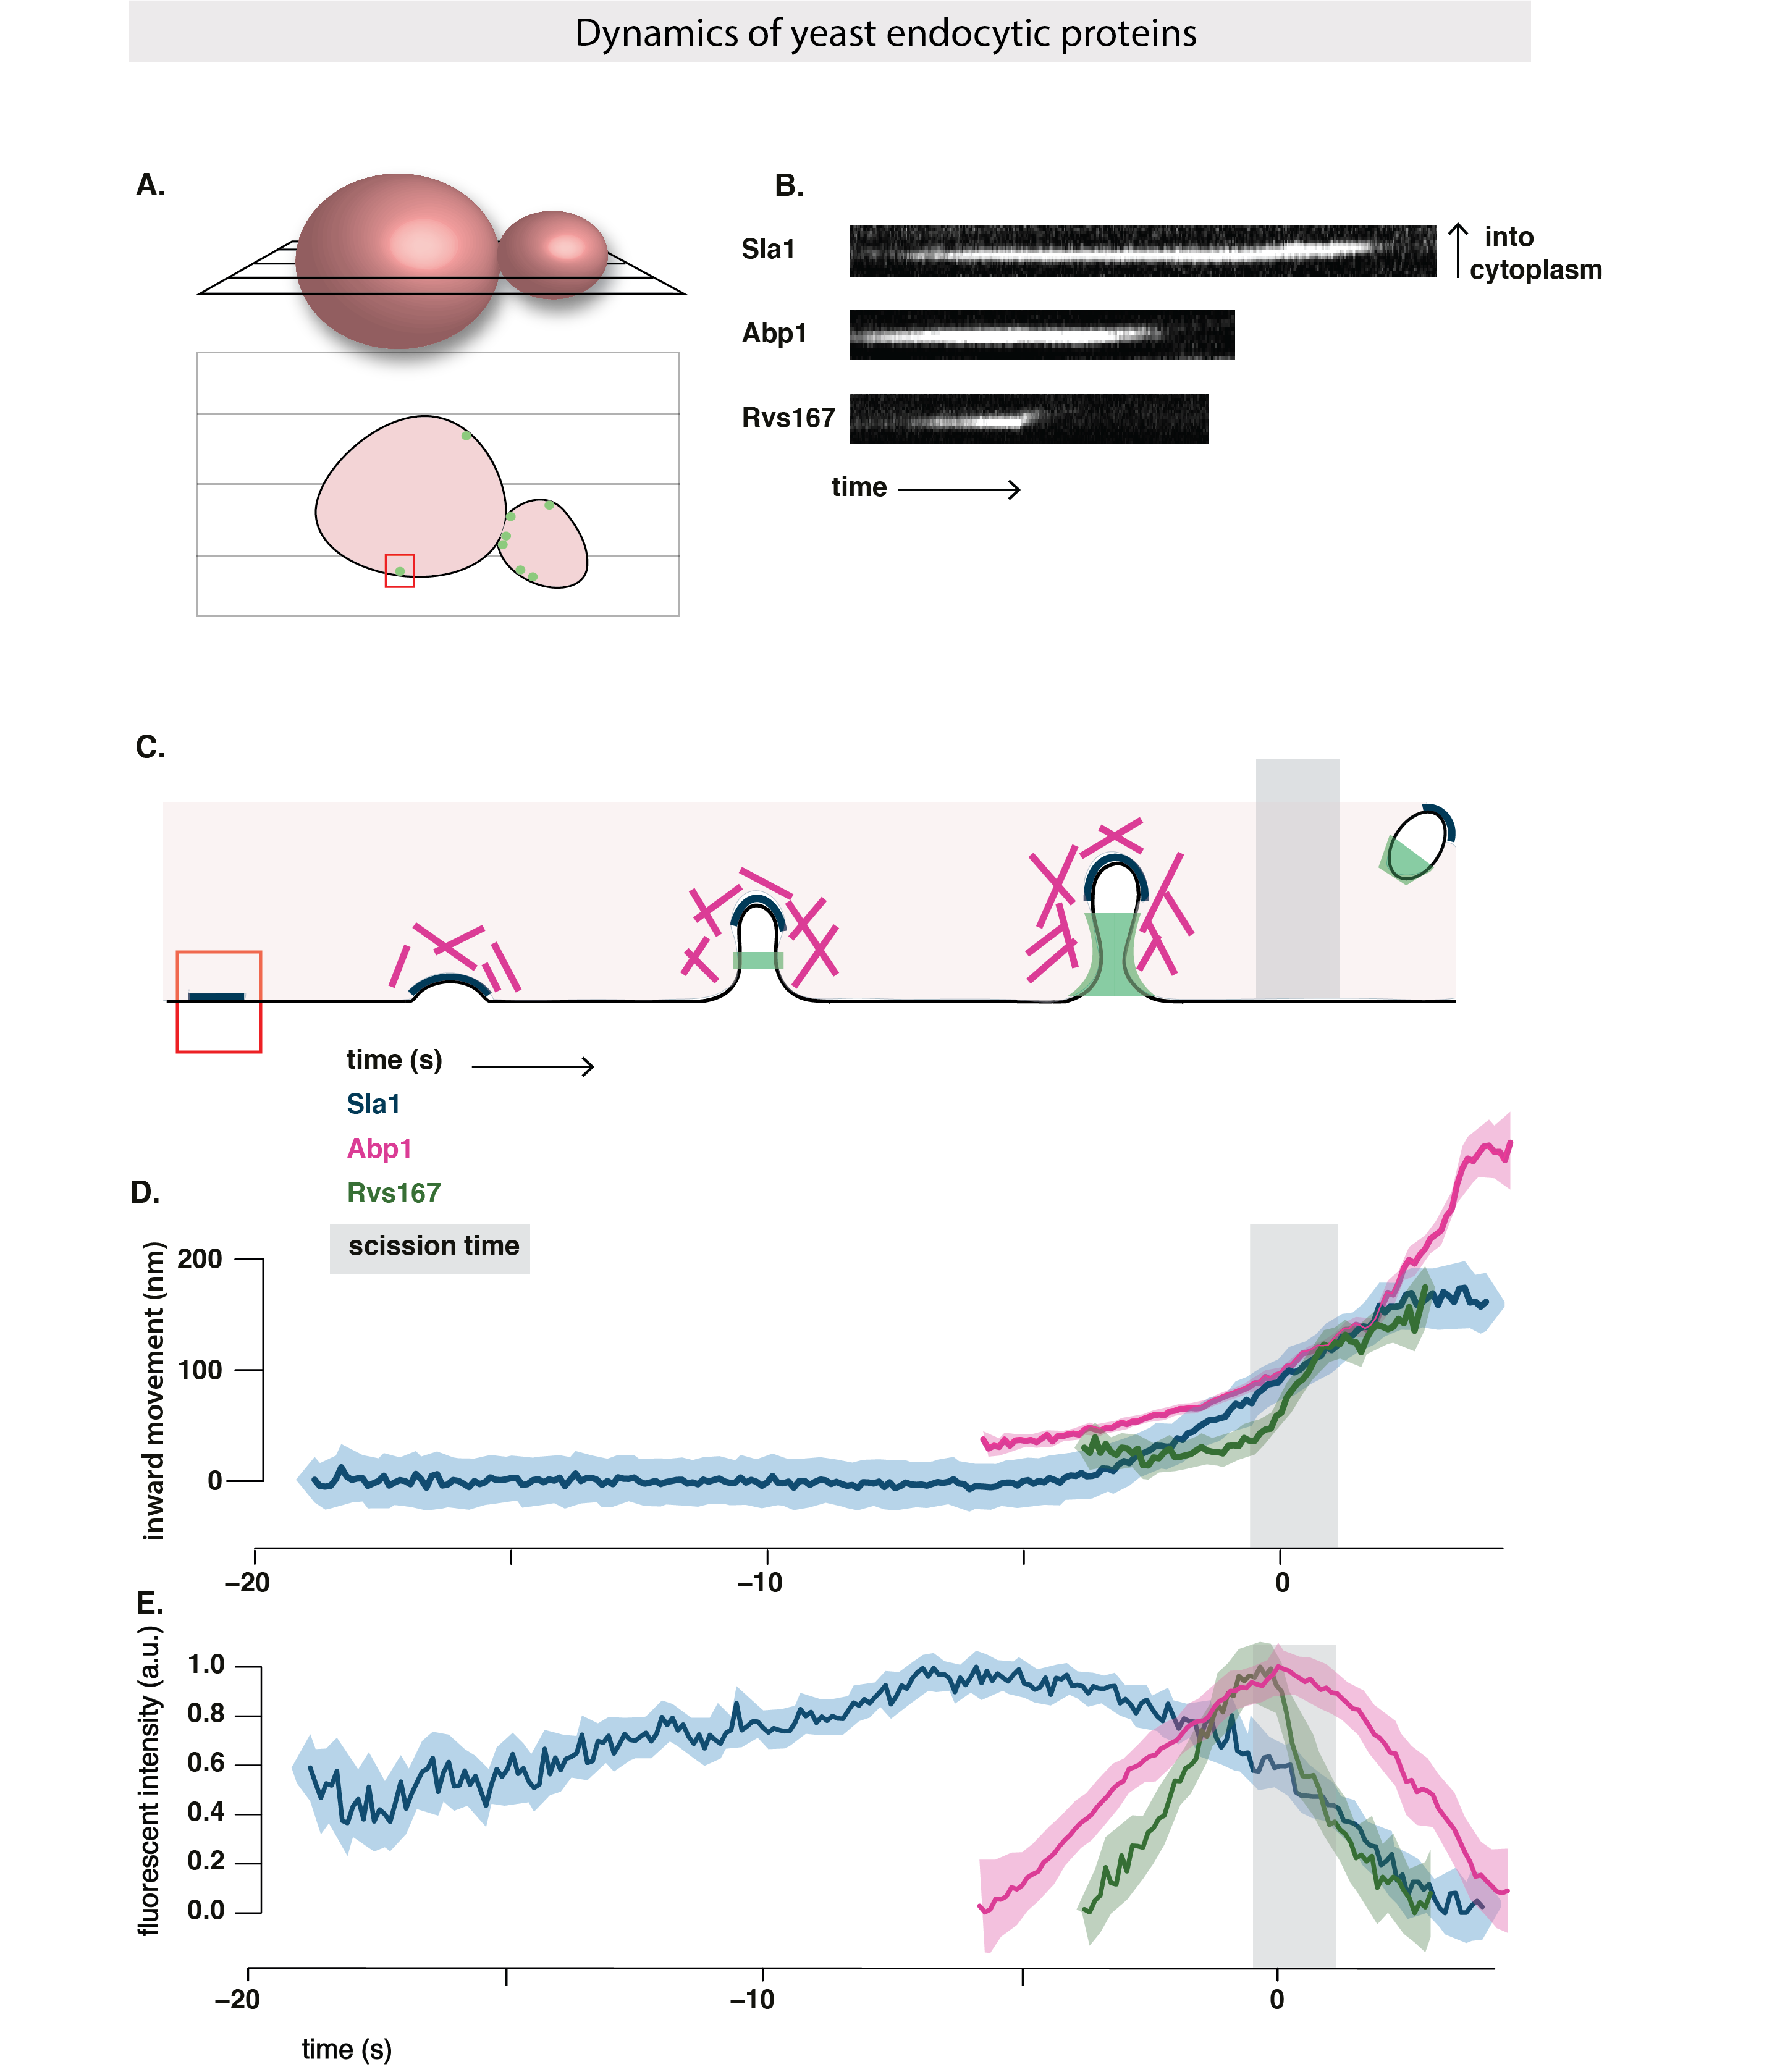
\includegraphics[width=21.5cm,height=21.5cm,keepaspectratio, valign=t]{figures/results_final/yeast_schemat_fig1_F}
	\caption[Centroid tracking yeast endocytic proteins]
	{Above: Schematic of a yeast cell, showing the equatorial plane. Below: Cross section of the cell at the equatorial plane, with fluorescently tagged endocytic protein at the plasma membrane. 
B: Kymographs of Sla1-GFP, Abp1-GFP and Rvs167-GFP at endocytic sites. Exposure rate 80ms.
C: Schematic of the timeline of membrane invagination during endocytosis, with Sla1, Abp1, Rvs167 and scission time (around 60\% of Rvs167 lifetime) indicated. 
D, E: Averaged centroid movement and normalized fluorescent intensity for Sla1, Abp1 and Rvs167. D and E are aligned in time so that time=0 (sec) corresponds to the maximum of fluorescent intensity of averaged Abp1 patches. This corresponds to scission time.

	
	\label{fig1_schematic}}
	\end{figure}



%rvs167$\Delta$ 
%\textit{rvs167$\Delta$}


\section{Rvs deletion phenotype}
\label{sec:rvsdel}

The Rvs complex, as has been discussed in \ref{Ch:Intro}, is known to have an influence on membrane scission efficiency. Recruitment in the final stage of membrane invagination, localization to the membrane tube, and disassembly concomitant with scission all indicate that Rvs could mechanistically influence the scission process.

	\vspace{2mm}
	
	\begin{figure}[H]
		\centering
		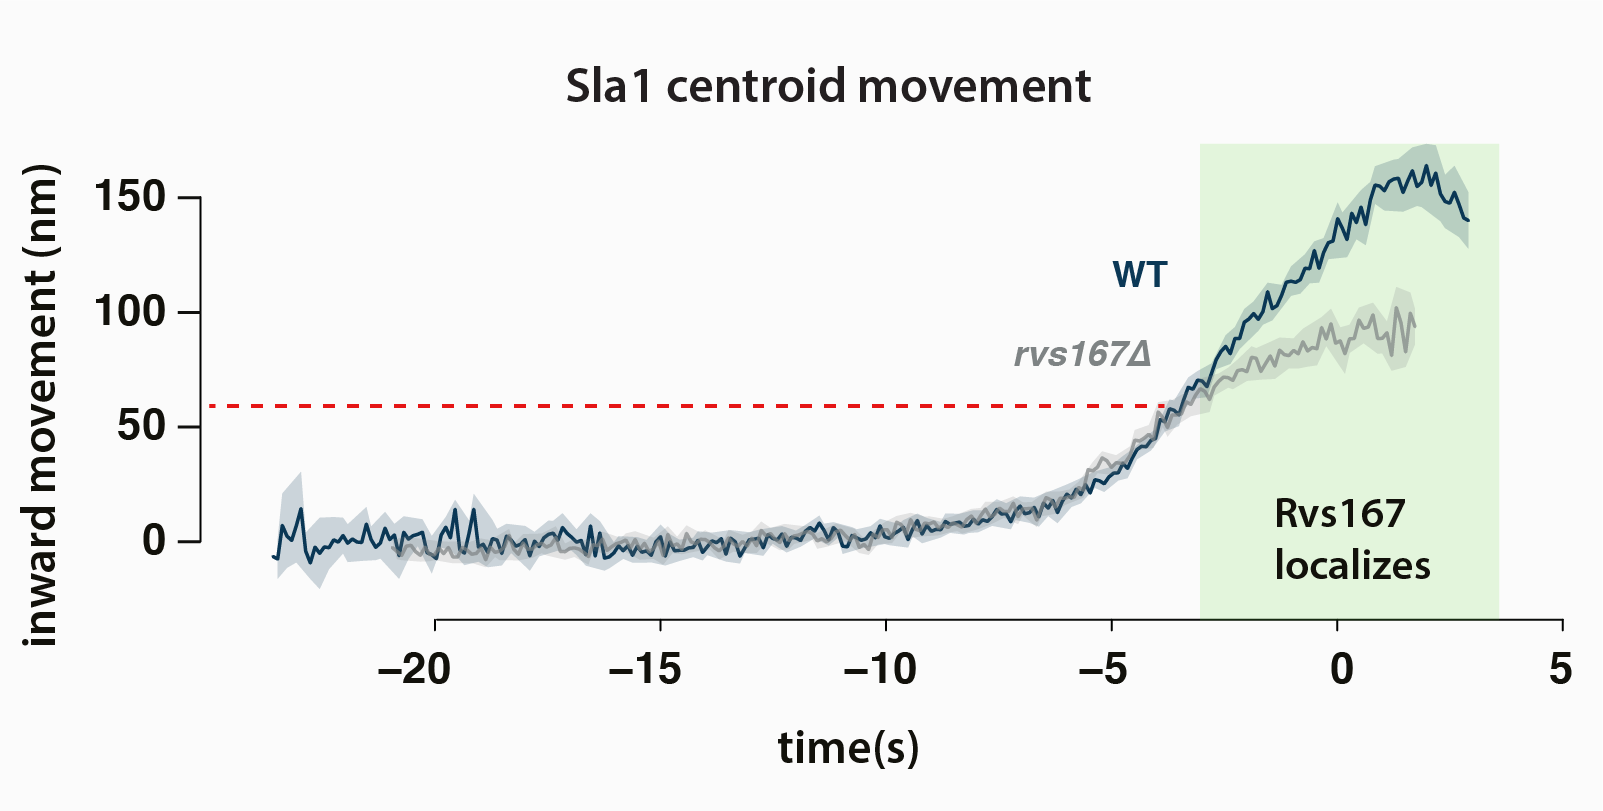
\includegraphics[width=14cm,height=19cm, keepaspectratio, valign=t]{figures/results_final/rvsdeletion3}
		\caption[some stuff]
		{Movement of Sla1-GFP in WT and  \textit{rvs167$\Delta$} cells. WT Sla1 is aligned in time so that time=0 (sec) corresponds to scission time. Averaged centroid of Sla1-GFP in \textit{rvs167$\Delta$} cells is shifted in time so that inward movement is concomitant with WT Sla1 movement. Red line indicates approximate start of deviation of \textit{rvs167$\Delta$} from WT. 
			\label{fig2_rvsdelta}
		}
	\end{figure}



	
In order to quantify what happens in the absence of Rvs, I tracked Sla1-GFP in rvs167Δcells and compared its movement against WT Sla1-GFP movement. 27\% of Sla1 patches begin to move inward but retract, consistent with earlier observations2. Movement of the remaining 73\% Sla1 patches are quantified. Sla1 movement of rvs167deletion and WT looks similar up to about 60nm. CLEM has shown that Rvs167 localizes to endocytic sites after the tubes are 60nm long. Sla1 movement in rvs167deletion shows therefore that membrane invagination is unaffected till Rvs is supposed to arrive. Sla1 in rvs167Δthen continues to move at a much slower rate, and membrane scission occurs at about 80nm. In WT, Sla1 continues to move inwards to 140nm. This indicates that first, membrane scission can occur at invagination lengths of 80nm. Then, that the arrival of Rvs prevents membrane scission at this point and allows further membrane invagination. 




%rvs167$\Delta$ 
%\textit{rvs167$\Delta$}

\section{Recruitment of Rvs and function of domains} 

	\subparagraph{Membrane curvature-sensing / generation by BAR proteins }
Cellular membrane shape is a result of properties like rigidity, tension, intracellular pressure, that are all influenced by membrane lipid composition and the proteins embedded in it 4,5. Since these properties all oppose membrane deformation, energy is required to deform and bend it. BAR domains localize to curved membranes, but they have also been shown to generate membrane tubes and cause vesicle formation, leading to some discussion on the interplay between these functions. 

	\vspace{7mm}
			
				\subparagraph{Membrane curvature-sensing / generation by BAR proteins }
BAR domains are thought to generate membrane curvature by either scaffolding or insertion of the N-helix into the lipid bilayer. 
Scaffolding refers interaction of the positively charged concave surface of BAR domains with negatively charged lipids. By attracting lipids to the positive surface, BAR domains are thought to induce membrane curvature. Curvature-generation by BAR scaffolding has been proposed as a function for I-BAR, F-BAR as well as N-BAR domains 6–10. 
	\vspace{7mm}
	
N-helices similar to that of NBAR domains can generate curvature independently of the BAR scaffold mechanism11,12. Shallow insertion of the N-helix into the upper lipid bilayer causes the bilayer to rearrange, and results in a difference in membrane surface area between the upper and lower leaflets13. This results in membrane curvature. 
	\vspace{7mm}
	
Sensing curvature:
BAR domains show preferential binding to membranes that correlates to their intrinsic curvature: flat F-BAR domain proteins are found at flat membranes, N-BAR domains are found at tubular structures1,14. That BAR domains are able to generate curvature does not imply that this is their function. In-vivo, the significance of curvature-generation is not determined. Tracking over thirty different endocytic proteins in NIH-3TC cells (derived from mouse fibroblasts), TIRF imaging shows that Endophilin2 and Amphiphysin1 arrive late in the endocytic time-line right before scission15, suggesting they arrive when membrane tubes are already formed. 

	\vspace{7mm}
Curvature-generation and sensing are likely intrinsically coupled mechanisms. BAR proteins that can induce curvature could also sense curvature: there could be feedback between membrane-sensing and generation. In the case of Rvs, that the complex localizes to sites after membrane tubes are formed shows that Rvs localizes once membrane curvature is established. Whether this localization is dependent on membrane curvature, recognized by the BAR domain is not known. 



	\subsection{BAR domains sense membrane curvature in-vivo}


To test whether Rvs is recruited because of membrane curvature, I tested the recruitment of Rvs167 without the BAR domain, that is Rvs167-delsh3 (henceforth BAR. Cells that contain Rvs167 without the SH3 domain are referred to as BAR cells). BAR-GFP forms cortical patches (Fig.3.2A), so the BAR domain is able to localize to the plasma membrane in the absence of the SH3 domain. In yeast cells expressing both BAR-GFP and Abp1-mCherry, BAR-GFP co-localizes with Abp1, indicating that BAR domains are recruited to endocytic patches (Fig3.2A, C). 

	\vspace{5mm}
In order to test whether this localization is due to membrane curvature, I compared the dynamics of Rvs167-GFP against BAR-GFP in sla2Δcells (Fig3.2D-F). Sla2 is a coat protein that acts as a linker between the membrane and actin cytoskeleton. It binds membrane via its N-terminal ANTH domain and actin by the C-terminal THATCH domain. This allows forces generated by the actin network to be transmitted to the membrane16. In sla2Δ cells, rather than cortical actin patches that co-localize to endocytic proteins, an “uncoupling phenotype” is observed16,17. Although endocytic coats are formed, actin is polymerized continuously at these sites, the membrane is not pulled inwards, and vesicles are not formed. Forces generated by the actin network are not transmitted to the membrane (Fig.2.2E).

	\vspace{5mm}
In sla2Δcells, Rvs167-GFP is recruited to the plasma membrane (Fig.2.2D,F), together with Abp1. Some Rvs167-GFP patches persist at the plasma membrane, while many are assembled and disassembled. In sla2Δcells expressing BAR-GFP, localization is removed except for rare transient patches at the plasma membrane. These patches rarely co-localized with Abp1. Rvs167-GFP and BAR-GFP patches are both dynamic, indicating an interaction exists in both cases that is able to assemble and disassemble Rvs molecules at the plasma membrane. 

	\vspace{5mm}
BAR-GFP is not typically recruited to the plasma membrane in sla2Δ cells, showing that the BAR domain requires membrane curvature to localize. 


% \textit{sla2$\Delta$} cells \ref{fig2_sla2del} (D-F). 

 
	\begin{figure}
	\centering
	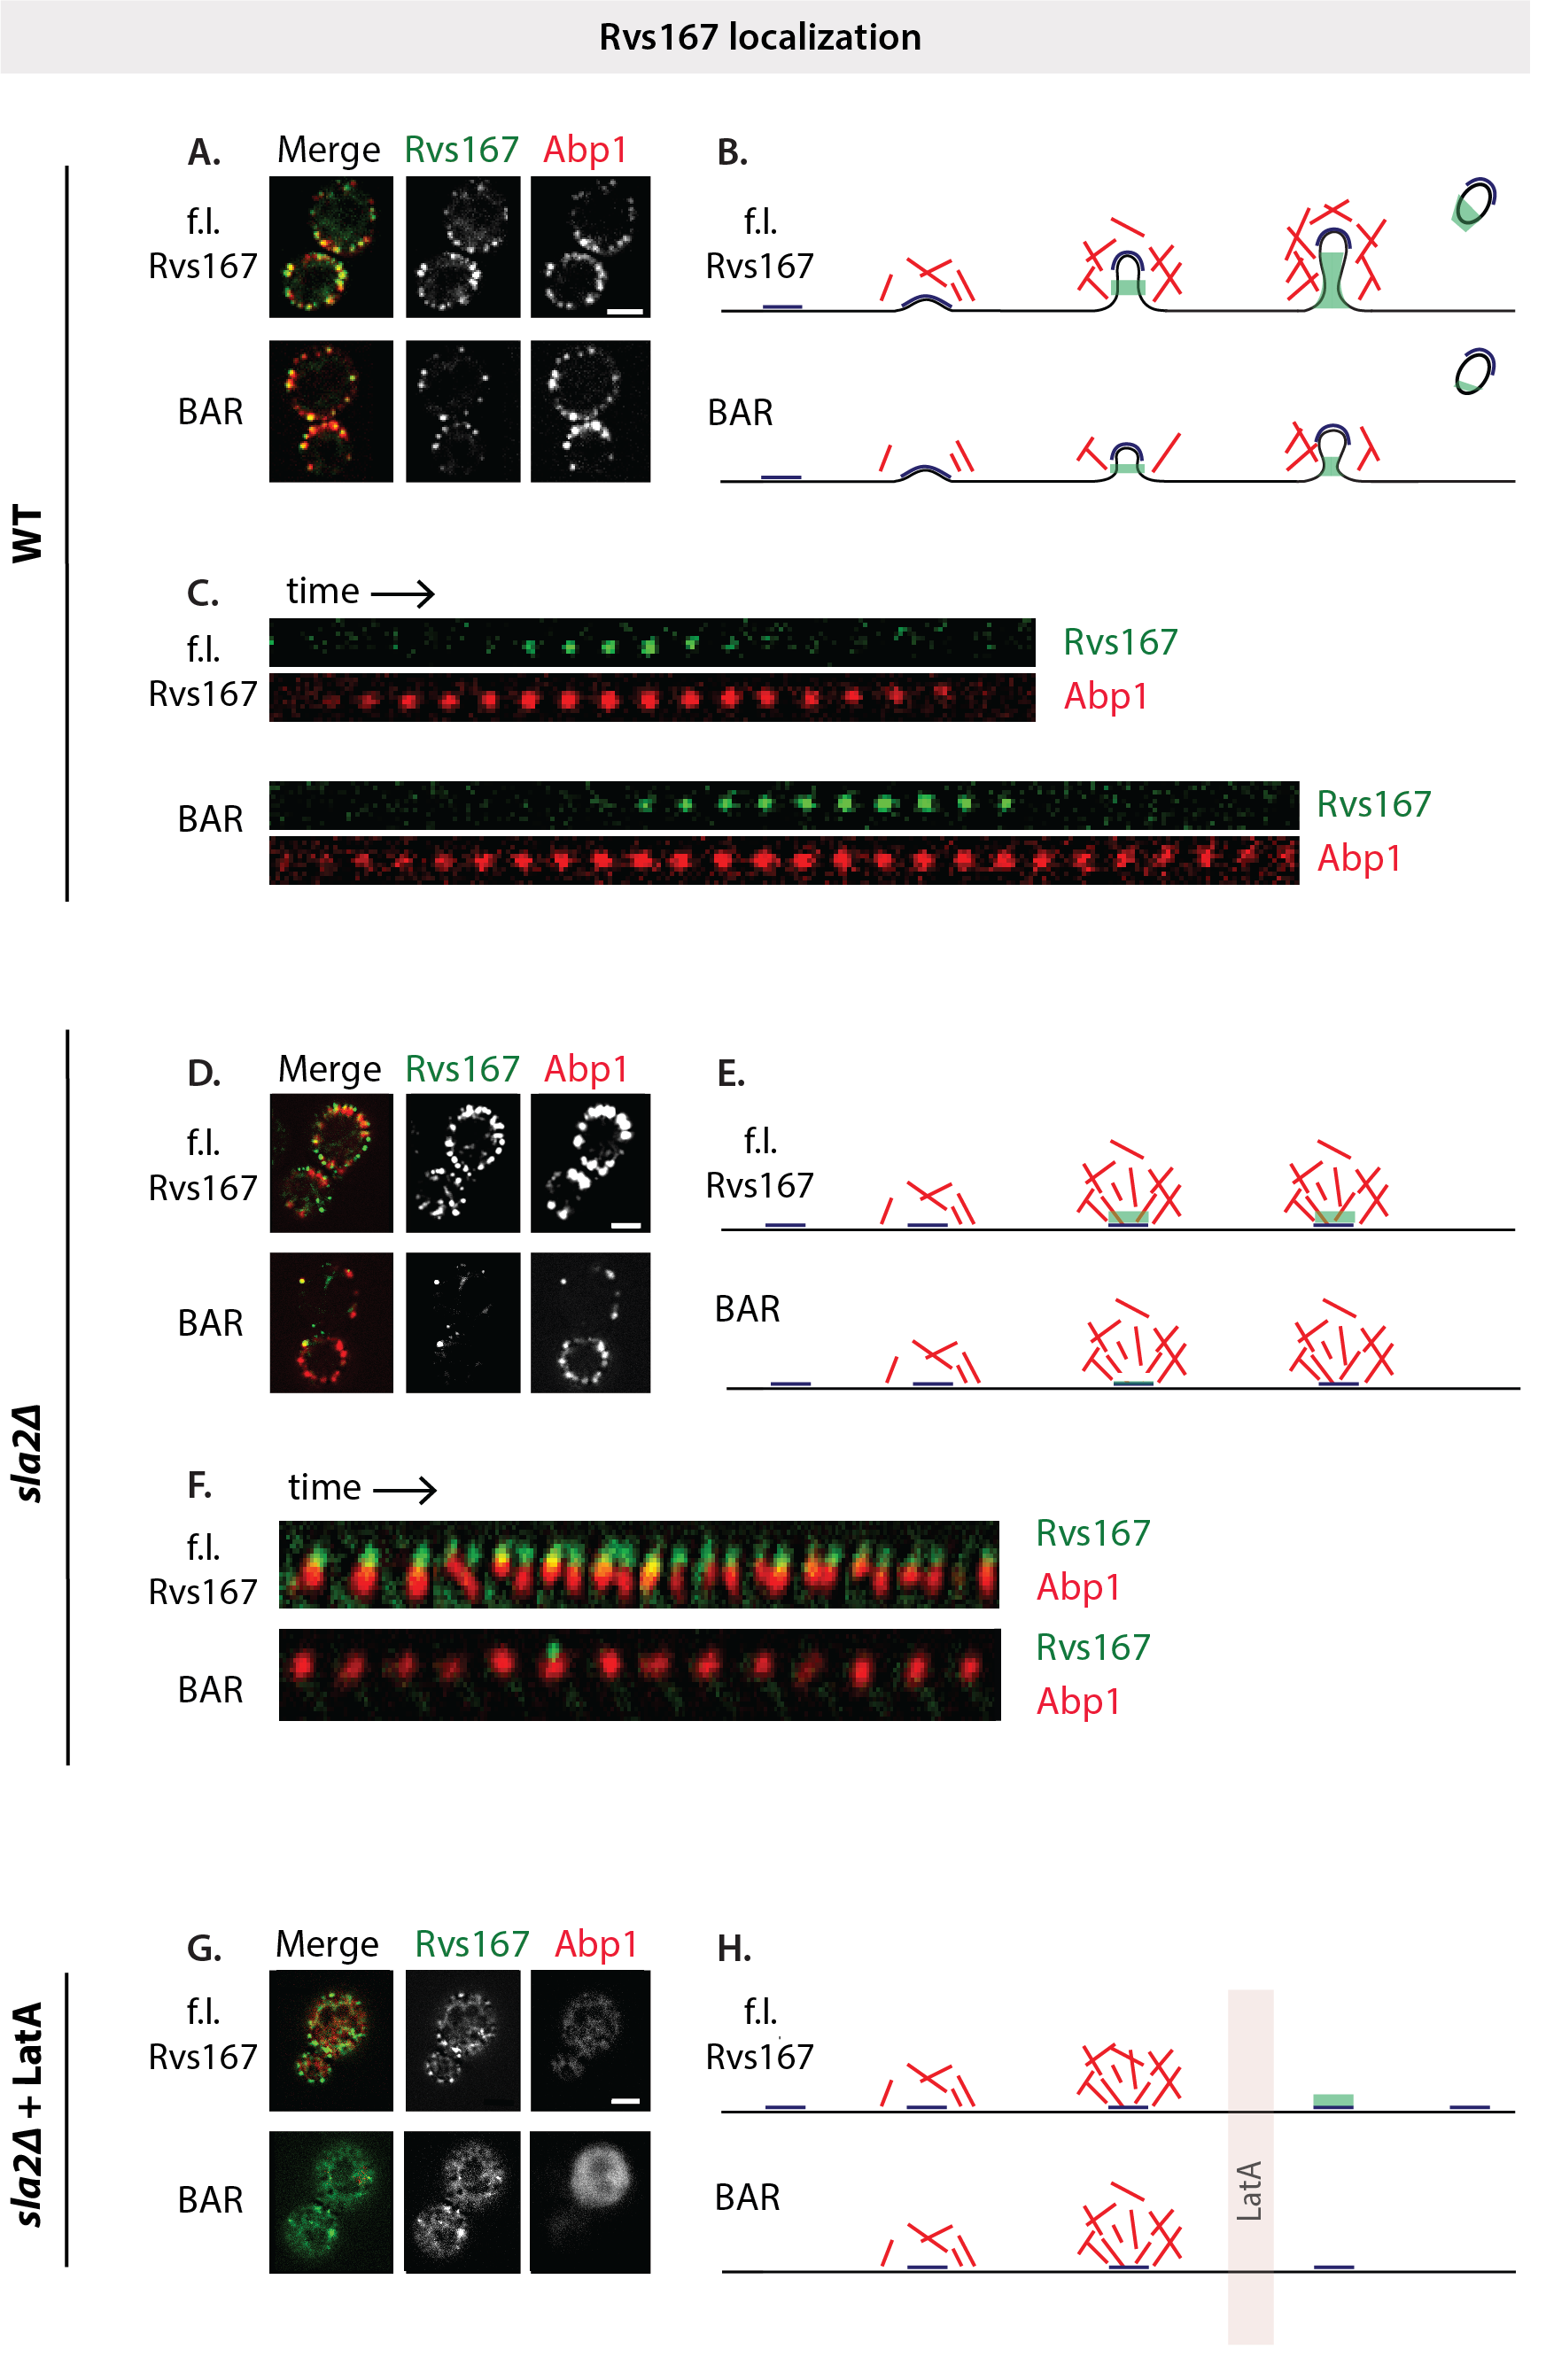
\includegraphics[width=21cm,height=21cm,keepaspectratio]{figures/results_final/sla2_del_final7}
	\caption [Localization of Rvs167 and BAR with and without membrane curvature]
{A: Maximum intensity projections of time-lapse images of Rvs167-GFP in WT and BAR cells, and Abp1-mCherry. Exposure time 250ms. B: Schematic of membrane progression of in WT and BAR endocytic events (BAR invaginations are shorter, and recruit fewer Rvs molecules: see section R1.3).
C: Montage of Rvs167-GFP in BAR and WT cells, and Abp1-mCherry. Time between frames= 750ms.
D: Maximum intensity projection of time-lapse images of Rvs167-GFP in  \textit{sla2$\Delta$} and \textit{sla2$\Delta$} BAR cells, and Abp1-mCherry. 
E: Schematic of membrane invagination in  \textit{sla2$\Delta$}. F: Montage of Rvs167-GFP or BAR-GFP with Abp1-mCherry. Exposure rate 1000ms for GFP, 800ms for RFP. 
G: Maximum intensity projection of time-lapse images of  \textit{sla2$\Delta$} cells expressing Rvs167-GFP or BAR-GFP, with Abp1-mCherry, after treatment with LatA for 10’. Exposure rate 1000ms for GFP, 800ms for RFP. H: Schematic of membrane invagination in sla2Δ cells treated with LatA. 
All scale bars = 2um.
	\label{fig2_sla2del}}
	\end{figure}



	\subsection{The SH3 domain is able to localize Rvs in an actin and curvature-independent manner}
	\label{delsh3_latA}
	As I show in the previous section, full-length Rvs is able to localize to cortical patches in \textit{sla2$\Delta$} cells. This As I show in R1.1, full-length Rvs167 is able to localize to endocytic patches in sla2Δcells. This localization must be dependent on the SH3 domain, since BAR alone does not localize in sla2Δcells. SH3 domains are known to interact many actin associated proteins: an interaction with Abp1 has been shown, as well as with Las17, type I Myosins, and Vrp1. 
	\vspace{5mm}
	
In order to test whether it interacts with an actin binding protein, I imaged BAR-GFP and full-length Rvs167-GFP in sla2Δcells treated with the actin sequestering agent LatrunculinA (LatA). LatA is a sea-sponge toxin that binds monomeric actin and prevents incorporation of actin into filaments. Since high actin turnover is required at endocytic sites, LatA effectively disassembles the actin network, and blocks endocytosis. In sla2Δcells treated with LatA, membrane curvature as well as actin-binding proteins are removed from endocytic sites. Loss of actin-binding proteins is observed by the loss of Abp1 signal.

	\vspace{5mm}
Surprisingly, full-length Rvs167 is transiently localized to the plasma membrane in sla2Δcells with LatA (Fig.2.2G, H). Localization occurs in the absence of a BAR-membrane interaction, since BAR-GFP patches are not seen in similarly treated cells. This suggests that the SH3 domain is able to recruit Rvs to the plasma membrane in the absence of curvature and actin network components. Rvs167-GFP patches are transient, so assembly and disassembly of an Rvs patch can be mediated by the SH3 domain. Localization of Rvs161, which does not have an SH3 domain, is removed by LatA treatment17, supporting the conclusion that the SH3 domain drives the localization of full-length Rvs167 in sla2Δcells, as well as in sla2Δcells with LatA. 



	\subsection{Loss of the SH3 domain affects progression of \\endocytic sites}
	\label{delsh3_movement}
The BAR domain was expected to act as the functional module of the Rvs complex: phenotypes of rvs167Δsuch as non-viability on starvation, and mis-localization of actin can be effectively rescued by expression of the BAR domain alone18. Since the SH3 domain unexpectedly influences localization of Rvs, I investigated its effect further.

	\vspace{5mm}
The SH3 domain generally mediates protein-protein interaction by binding to proline-rich sequences that contain a core PXXP motif19,20 (where X is any amino acid). These domains are ubiquitous in cellular interaction pathways, and several endocytic proteins have at least one SH3 domain. Although SH3 domains are abundant, they appear to have specific binding partners that could modulate function. For Rvs167, neither binding partner, nor function of the SH3 domain is clear. 

	\vspace{5mm}
In order to probe the contribution of the Rvs SH3 domain to endocytosis, I studied Sla1 and Rvs167 in BAR cells, and quantified the number of molecules recruited to endocytic sites as in Picco et al.,1. Fig. 2.3C shows that recruitment of Rvs167 is reduced by half (57 +/- 9.9 for BAR compared to 113.5 +/- 5.3 for WT). Cytoplasmic concentration of Rvs167 appears not to be different in WT vs BAR cells (see methods). The inward jump of Rvs167 is reduced in BAR cells compared to WT (Fig.2.3A). Movement of the coat protein Sla1 is similarly reduced (Fig.2.3A). Sla1 moves into the cytoplasm approximately 60nm instead of the 140nm found in WT invaginations. Abp1 recruitment in BAR cells is reduced to 50\% of WT recruitment, to 172.6 +/- 12.9 from 347+/- 30.6 molecules in WT (Fig.2.3C). Short invaginations with a maximum of 60nm have been observed in the case of Rvs167 deletion by CLEM3, which is about the same length as those observed in the SH3 deletion: loss of the SH3 domain appears to be detrimental to the function of the Rvs complex. That tubular invaginations are formed in BAR cells, and qualitatively resemble that in WT cells is demonstrated by CLEM on WT and BAR samples expressing Rvs167-GFP and Abp1-mCherry (Fig.2.3E). 

	\vspace{5mm}
To check if there was a change in the timing of endocytic progression, I quantified the lifetimes of Rvs167, Sla1 and Abp1 in BAR cells using total internal reflection fluorescence (TIRF) microscopy. Unlike epifluorescence microscopy at the equatorial plane, in TIRF only fluorophores up to a depth of about 100nm from the glass-sample interphase are excited. This reduces fluorescent signal from the cytoplasm, allowing detection of low intensity fluorescent signal, and is a better method for quantification of protein lifetime than epifluorescence microscopy. Although this method is sensitive to low fluorescent intensity, as the proteins start to move inwards into the cytoplasm, fluorescent intensity rapidly drops, because of the limited excitation depth. Therefore, rather than a quantification of the entire lifetime of the protein, this is a quantification of the non-motile lifetime of a protein that arrives at endocytic sites. Non-motile lifetimes of Rvs167, Sla1 and Abp1 are thus compared between BAR and WT cells. 

	\vspace{5mm}
While lifetimes of Rvs167 and Sla1 are similar in both cell types, there is a significant increase in the lifetime of Abp1 in BAR cells (supplemental). Increase in lifetime of Abp1 is also seen by epifluorescence microscopy (Fig.2.3B). I then looked for differences in the sequence of recruitment of these proteins by looking at the difference in time between recruitment of Sla1 and Rvs167, and the difference in time between recruitment of Abp1 and Rvs167. The time difference between recruitment of Sla1 and Rvs167 is unchanged between WT and BAR cells, while the difference in time between recruitment of Abp1 and Rvs167 is increased in BAR cells (Fig.2.3D).

	\vspace{5mm}
This data suggests that the BAR domain alone cannot reproduce the function of the Rvs167 at endocytic sites: recruitment of Rvs, coat and actin dynamics are all affected. 



\begin{figure}
	\centering
	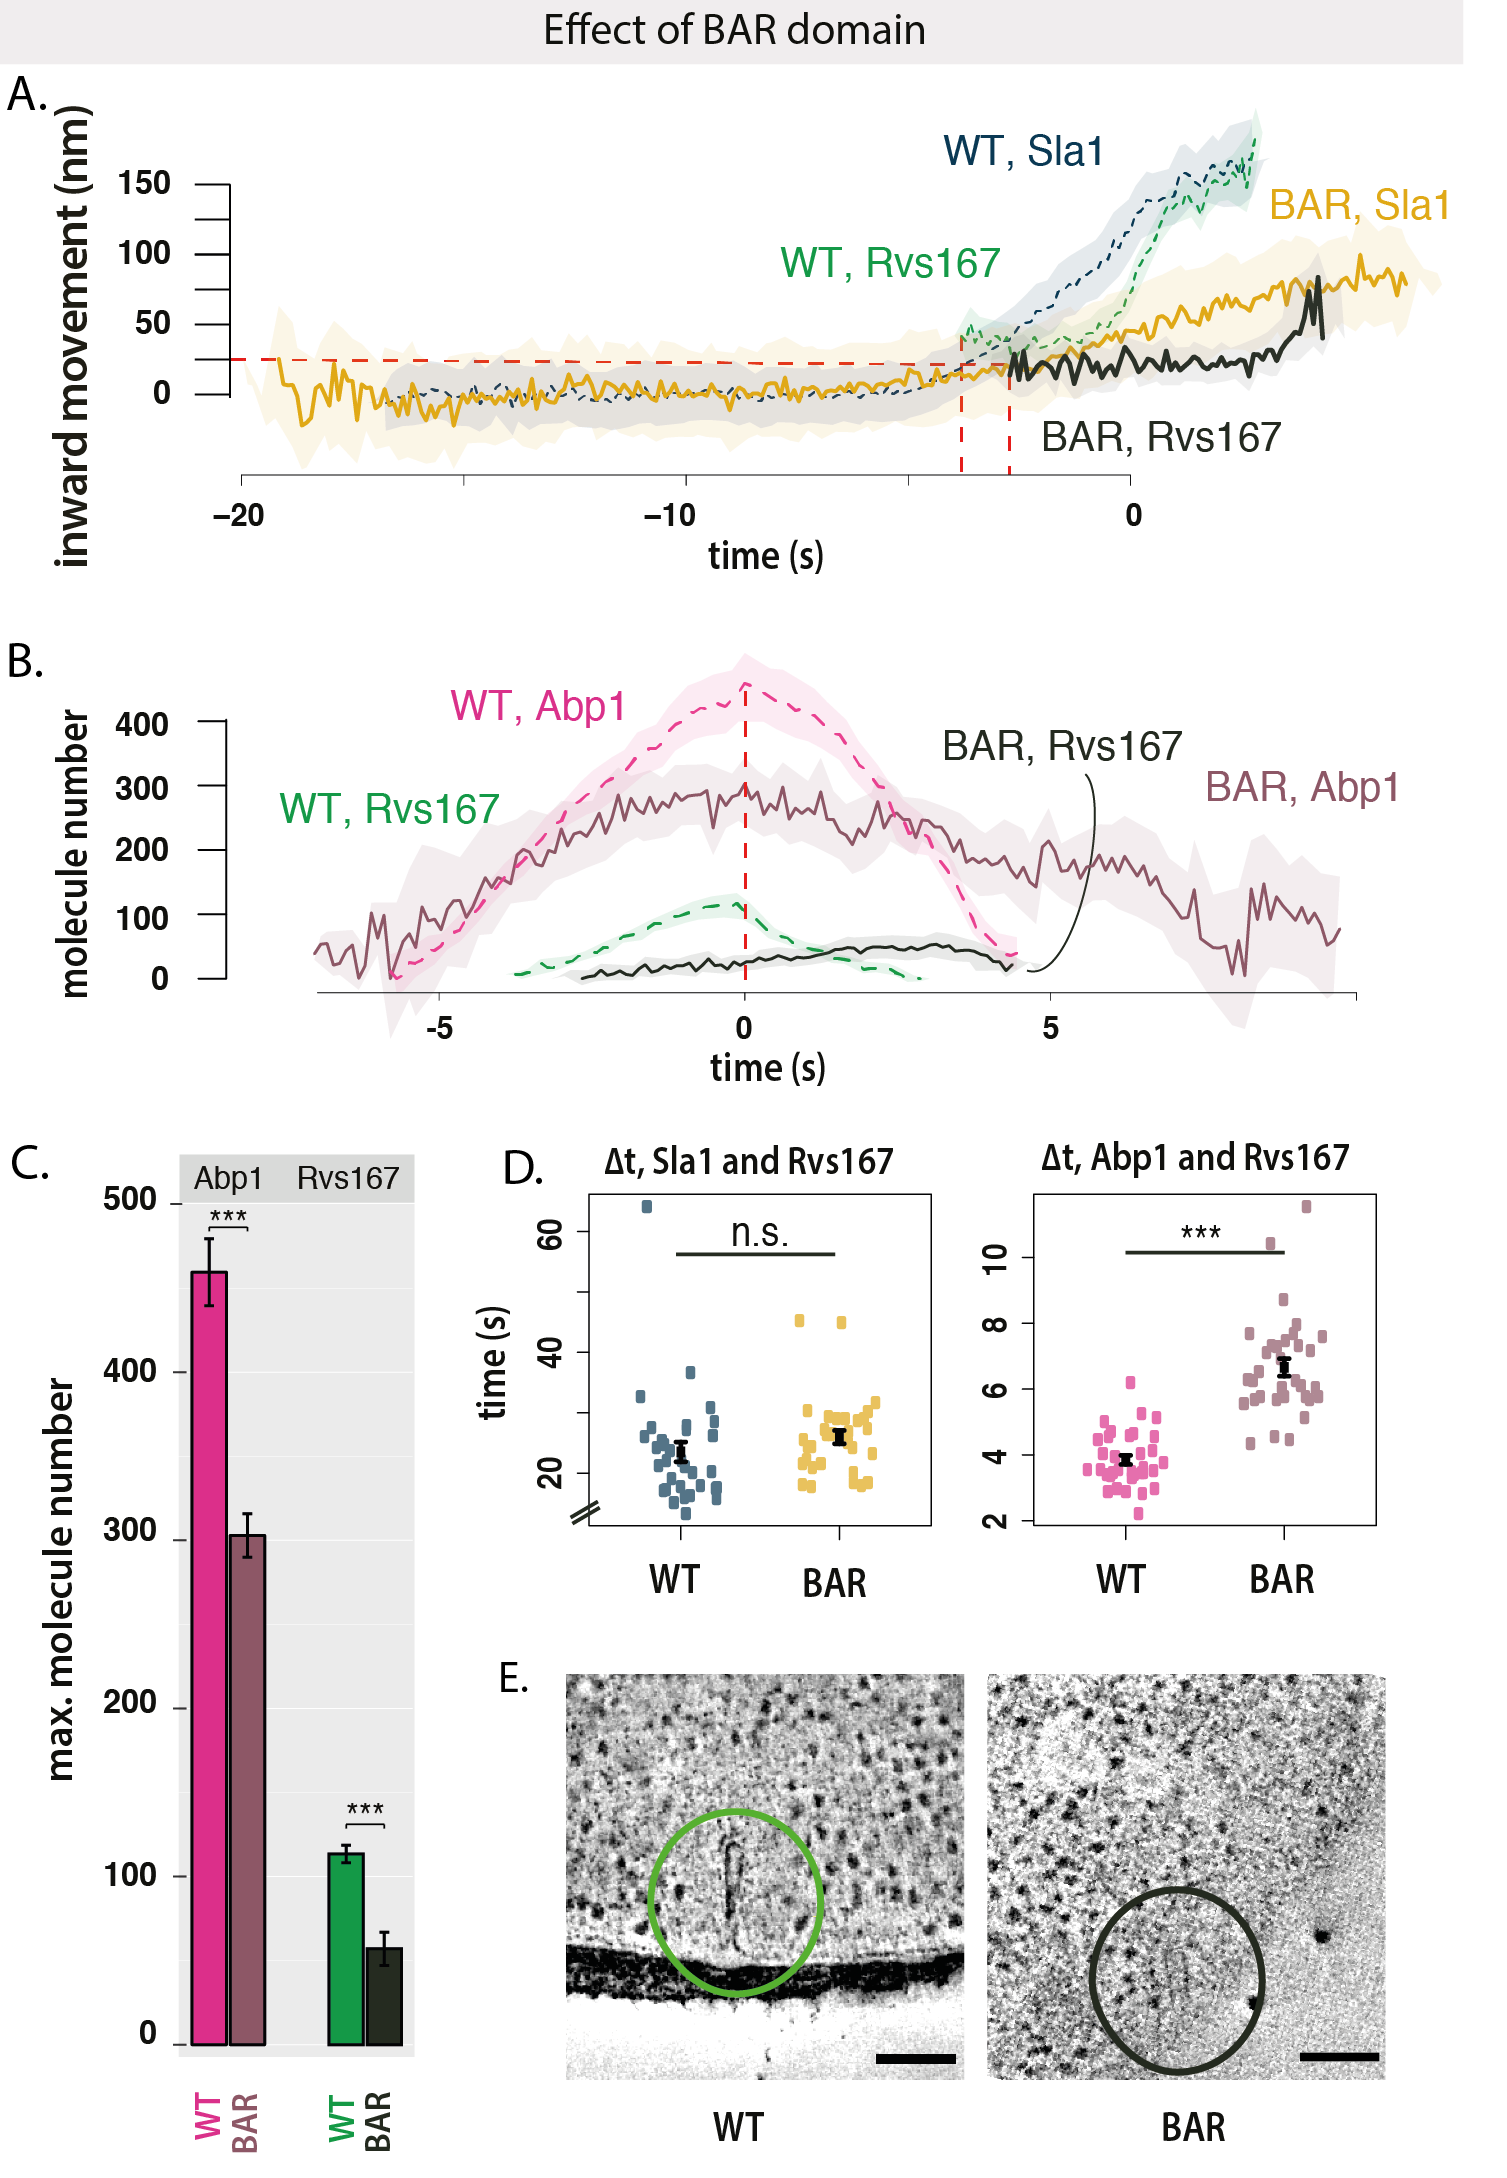
\includegraphics[width=21cm,height=21cm,keepaspectratio]{figures/results_final/delsh3_8}
	\caption [Effect of the Rvs167 SH3 deletion]
	{A: Movement of Sla1 and Rvs167 in WT and BAR strains. Centroids are aligned in time so that time=0 corresponds to the Abp1-mCherry fluorescent intensity peak in simultaneous dual-color imaging of the corresponding strains. 
	C: Maximum number of molecule of Abp1-GFP in WT, and BAR cells, and Rvs167-GFP in WT and BAR cells, with standard error of mean. p values from a two-sided z test, * = p $\leq$ 0.05 , ** = p$\leq$ 0.01, *** = p $\leq$ 0.001. 
	D: Difference in time between arrival of Sla1-mCherry and Rvs167-GFP, and Abp1-mCherry and Rvs167-GFP in WT and BAR strains. Exposure 560ms for each channel. Mean and standard error of the mean are shown, * = p$\leq$ 0.05, ** = p$\leq$ 0.01, *** = p$\leq$ 0.001. p values of two-sided t test.
	E: Invagination lengths in WT and BAR cells measured by CLEM in cells expressing Rvs167-GFP and Abp1-mCherry. 
	\label{fig2_sh3del}}

	\end{figure}
	\vspace{5mm}
	
		
\section{Function of Rvs}

	\subsection{BAR domains as scaffold for dynamin}
	\subparagraph{Yeast dynamin Vps1}
	
While work on membrane scission in mammalian cells has converged on the idea that it is caused by dynamin interaction with BAR domains, in yeast what causes the final shape-transition from tubes to vesicles is not determined. Several membrane scission mechanisms for yeast endocytosis have been proposed in the last years, in the absence of conclusive mechanistic evidence. We know that Rvs plays a major role in determining the efficiency of membrane scission, and that in its absence membrane invaginations are shorter than in WT. I have therefore focused of models for membrane scission that assign a central role to BAR domain proteins. In the following pages, I discuss their propositions, describe experiments that have tested these mechanisms, and the conclusions they propose. 

	
		\subparagraph{Rvs as an interaction surface for dynamin }
	\mbox{}\\
Yeast dynamin is the obvious solution to membrane scission. None of the three dynamin-like yeast proteins has a proline-rich domain that are known to bind BAR domains, but one of them- Vps1 has been suggested to function like the mammalian homologue 21,22. Rooij et al., propose that Vps1 localizes to endocytic sites at scission stage, and see that in vps1Δrvs167Δ cells, rates of coat retraction after invagination increases. Coat retraction after invagination is an indication of membrane scission failure2. Vps1-GFP does not localize to endocytic sites in Gadila et at.,23, but localizes to the golgi body and to vacuoles. Kishimoto et al24, do not find a co-localization between Vps1 and Abp1, and find that the vps1Δ rvs167Δ  cells do not show increased coat retraction rates. Vps1 tagged with GFP as well as superfolded GFP, and imaged by TIRF microscopy fails to co-localize with Abp1 (data from Andrea Picco, not shown). The debate concerning the involvement of Vps1 in membrane scission in yeast has been compounded by the possibility that the GFP tag on Vps1 could interfere with its localization to endocytic sites, and/or its interaction with the Rvs complex. 

	\vspace{5mm}
If Vps1 was required for membrane scission, Sla1 would be expected to undergo delayed or failed scission in its absence, and Rvs dynamics would be affected. 

	\begin{figure}
	\centering
	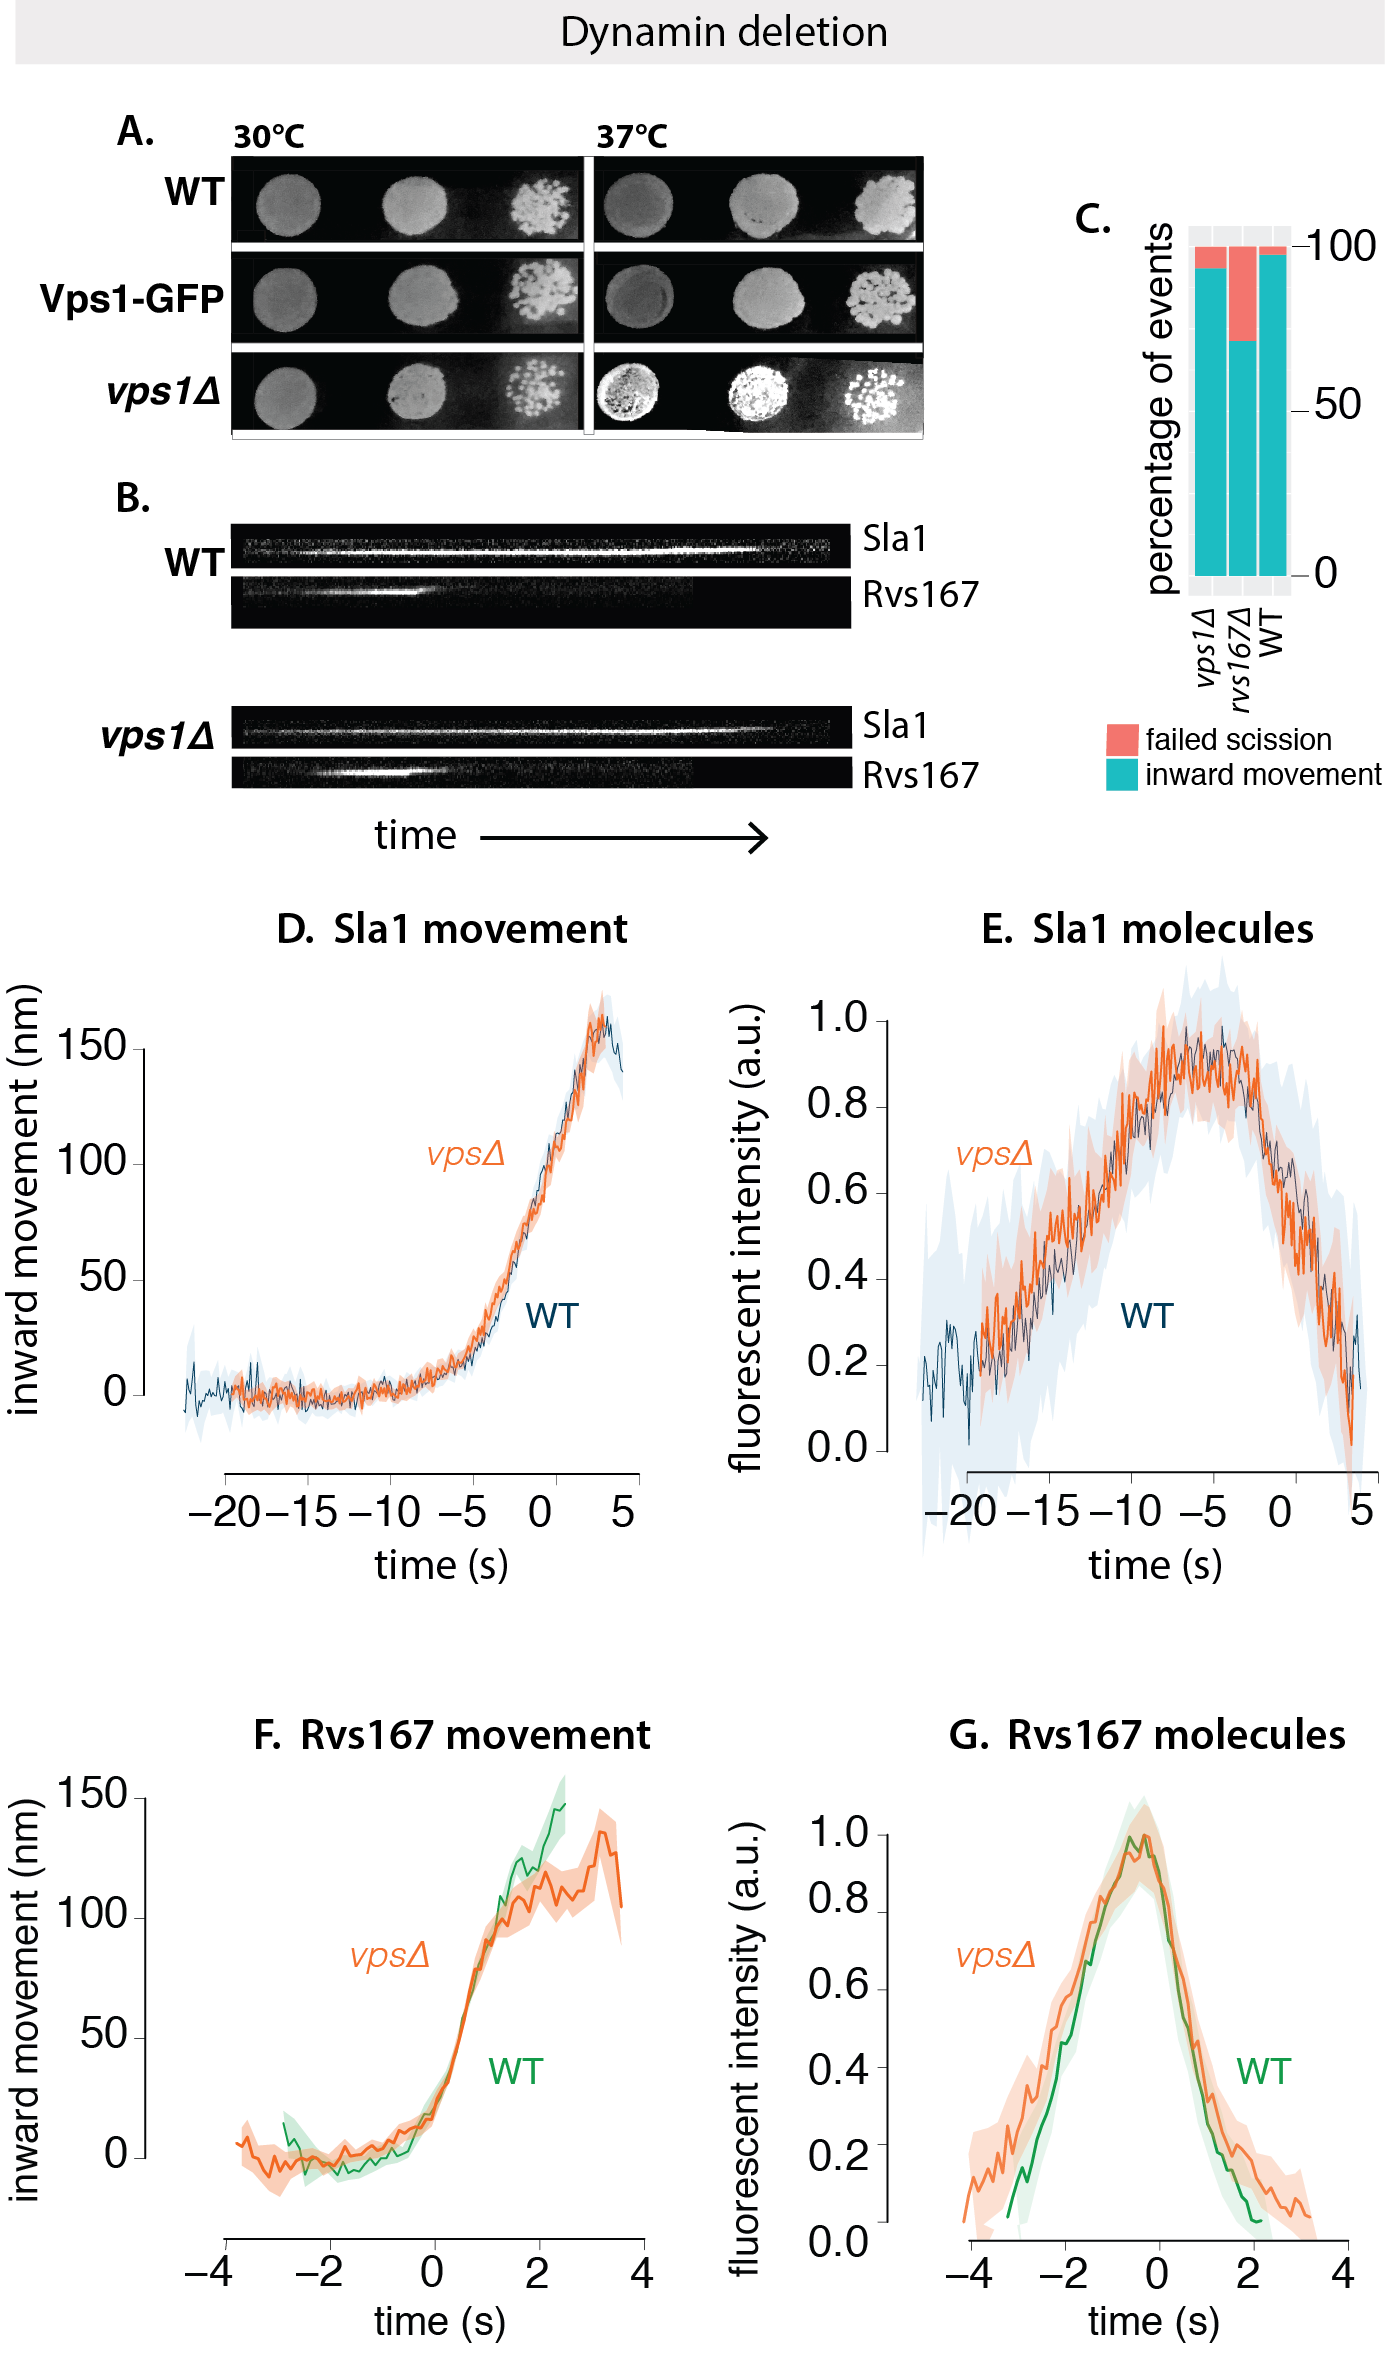
\includegraphics[width=22cm,height=22cm,keepaspectratio]{figures/results_final/vps}
	\caption[Rvs localization in vps deletion]
	{A: Dot spots of WT, Vps1-GFP, and \textit{vps1$\Delta$} cells at 30C and 37C. 
		B: Kymographs of Sla1-GFP and Rvs167-GFP in WT and \textit{vps1$\Delta$}. Exposure 80ms.  
		C: Failure rate of membrane scission, measured from retractions of Sla1, or lack of movement. 
		D, E: Movement and normalized fluorescent intensity of Sla1-GFP in WT and \textit{vps1$\Delta$} cells. Time =0 (s) for WT Sla1 indicates scission time. \textit{vps1$\Delta$} Sla1  is shifted to move inwards at the same time as WT. 
		F, G: Movement and normalized fluorescent intensity of Rvs167-GFP in WT and \textit{vps1$\Delta$} strains. Time =0 (s) for WT Rvs167 indicates scission time. \textit{vps1$\Delta$} Rvs167 is shifted so that fluorescent intensity maxima is at time=0 (s).
		\label{fig4_vpsdel}}
	\end{figure}
	
			\subsubsection{Vps1 does not affect Sla1 or Rvs167 dynamics }
	\vspace{5mm}
%	\textit{vps1Δ }
I investigated the role of Vps1 by studying coat and scission proteins in vps1Δ cells in order to avoid the question of whether fluorescently tagging Vps1 affects its function. 

vps1Δ cells exhibit a growth defect at 37C, as has been reported21. In vps1Δ cells, Sla1 accumulates in patches at the plasma membrane, moves inwards, and disassembles like in WT. vps1Δ does not increase the rate of membrane retraction (Fig.2.5C). Centroid movements and intensities of Sla1 and Rvs167 in time are plotted in Figure2.5D-G. WT Sla1 is aligned so that time=0 (s) corresponds to scission time. Sla1 movement for vps1Δ in Fig.2.5D is shifted in time so that it starts to move inwards at the same time as WT. The lifetime of Sla1-GFP appears to be slightly shortened in vps1Δ compared to the WT, but this shortening occurs early in the lifetime of the protein at endocytic patches, when the molecule numbers of Sla1 are low. Epifluorescence microscopy is not particularly sensitive in this range of fluorescent intensity. Therefore, I do not take this to indicate a true shortened lifetime; lifetime of Sla1 in vps1Δ was not investigated further. Similar to WT, Sla1 in vps1Δ moves into the cytoplasm about 140nm before membrane scission occurs. Sla1 moves inward at the same rate, and to similar maxima as WT. 

Dynamics of Rvs167 also remains the same as in WT (Fig.2.5F,G). Magnitude of centroid movement is unchanged, indicating that the base of the vesicle formed is likely at the same position as in WT. Fluorescent intensity shows the typical sharp drop. This data indicates that if Vps1 is localized to endocytic patches in S.cerevisiae, it is not involved in regulating membrane scission.  

	\subparagraph{ LRvs forms a barrier for lipid diffusion, generating forces for scission
}
Phosphatidylinositols (PIs) and their lipid derivatives play important roles in many cellular processes including membrane trafficking and cell signalling. Conversion between lipid types is driven by kinases, lipases, and phosphatases and controlled throughout the membrane trafficking pathway. 

Phosphatidylinositol (4,5)-biphosphate (PI(4,5)P2) is an important lipid type found at the cell surface, and is enriched and depleted from endocytic sites at the plasma membrane in concert with the assembly and disassembly of the endocytic machinery. Synaptojanins form a subset of inositol polyphosphate 5-phosphatases that hydrolyze PI(4,5)P2 to PI(4)P by removing the phosphate at the 5’ position of the inositol ring. They are known to take part in CME and intracellular signalling, as well as in modulating the actin cytoskeleton25. 

In mammalian cells, disruption of Synaptojanin genes results in cellular accumulation of PI(4,5)P2 at endocytic sites. Coated vesicles gather at the plasma membrane, suggesting a role for lipid hydrolysis in releasing coat proteins from nascent vesicles. Synaptojanins contain an N-terminal homology domain with the cytoplasmic domain of the yeast SAC1 gene that is implicated in lipid metabolism, actin morphology, and vesicle transport in the secretary pathway26. A central catalytic domain is then followed by a proline-rich C-terminal region that is the canonical interaction partner of SH3 domains. Synaptojanins interact with actin binding proteins and BAR domain proteins, potentiating also a role in membrane invagination and scission. 

The yeast genome encodes for three Synaptojanin-like proteins- Inp51, Inp52 and Inp53- that regulate phospholipid metabolism. In inp51Δ inp52Δ cells, increased lifetimes of endocytic proteins and produce aberrant membrane invaginations that could indicate scission failure and defective endocytosis27,28. inp52Δ rvs167Δ cells have increase membrane retraction rates, supporting a possible role for Inp52 in membrane scission24. Loss of inp51 leads to an increase in bulk PI(4,5)P2 level. Changes in PI(4,5)P2 levels have not been reported for mutations of Inp52, and are lipid levels not measured locally at the endocytic sites29,30.

In a moΔproposed by Liu et al, Synpatojanins and BAR proteins interact to regulate PI(4,5)P2 hydrolysis, which in turn drives membrane scission. Here, Rvs forms a scaffold on the membrane tube, and protects the underlying PIP2 from hydrolysis. Synaptojanin arrives at inavaginated membranes, and hydrolyses unprotected PIP2. This generates a boundary between BAR-protected PI(4,5)P2 at the tube and PI(4,5)P at the bud tip. This lipid boundary produces line tension at the interphase that could generate enough force to pinch off a vesicle. 

The Liu et al., moΔpredicts that if line-tension from lipid hydrolysis is removed, membrane scission should be delayed or fail.


	\subsection{Yeast synaptojanins do not significantly affect coat and Rvs movement } 

	
	
I tested the lipid hydrolysis moΔdescribed above by studying the effect of synaptojanin deletion on Sla1 and Rvs167. 

Of the three yeast Synaptojanins, only Inp52-GFP localizes to cortical patches (Fig.2.6D). Time alignment with other endocytic proteins as in Picco et al., shows that Inp52 localizes to endocytic sites at the late stage of scission, similar to Rvs. The centroid of Inp52-GFP can be localized to the tip of the invaginated tube (Fig.2.6D), consistent with the Liu theory of membrane scission: spatial and temporal localization is consistent with influence on scission. Inp51-GFP exhibits a diffuse cytoplasmic signal, while Inp53 localizes to patches within the cytoplasm, likely to the trans-golgi network, as has been noted in other work31. 
	\vspace{5mm}
	
In both inp51Δ and inp52Δ cells, Sla1-GFP patches are assembled and disassembled, as is Rvs167-GFP. Sla1 retraction rates are slightly increased to 12\% in inp52Δ, compared to 2\% in WT, and 6\% in inp51Δ (Fig.2.7B). In Fig.2.7A, Sla1 movement in inp51Δ and inp52Δ cells is compared against that in WT. WT Sla1 is aligned in time so that time=0 (s) corresponds to scission time. Sla1 centroids for inp51Δ and inp52Δ are shifted so that they begin to move inwards at the same time as the WT. All three Sla1 centroids have the same rate of inward movement. While Sla1 in inp51Δ moves inwards to about the same distance as WT, in inp52Δ, the centroid of Sla1 persists for nearly 5 seconds longer than WT (arrowhead in Fig.2.7A). This centroid movement is noisier than the inward movement preceding it, and is likely from post-scission of movement of the vesicle. 
	\vspace{5mm}
	
Rvs167 dynamics are similar to WT in both inp51Δ and inp52Δ cells (Fig.2.7C, D). Rvs167 centroids move inwards to about the same distance into the cytoplasm at the jump inwards. In inp52Δ cells, however, Rvs167 patches appear to not disassembly completely (arrowhead in Fig.2.7C) unlike in the WT. Since Rvs disassembly occurs at membrane tube scission, this change in Rvs167 dynamics is post-scission. Assembly of Rvs167 in the inp51Δ takes about 2 seconds longer compared to WT. The implication of this delay is not thus far clear. 
	\vspace{5mm}

Since the differences in Sla1 and Rvs167 centroid dynamics for inp52Δ are post-scission, I find that the data is consistent with a role for Inp52 in removing Sla1 and Rvs167 from vesicles, rather than a primary role in membrane scission. 




	
I then quantified the number of Rvs167 molecules recruited to endocytic patches in inp51Δ , inp52Δ, and inp51Δ inp52Δ cells.  WT levels of Rvs167 are recruited in both inp51Δ and inp52Δ cases. In inp51Δ inp52Δ however, nearly three times as much Rvs is recruited to sites. Some Rvs167-GFP patches in these cells assemble and disassemble, although majority do not. Many large clusters of Rvs167 are present on the plasma membrane, and the regular inward jump in WT is not seen. Some cytoplasmic patches are also seen, consistent with observations of Sla1 patches within the cytoplasm32 by other labs. These patches likely mark aberrant membrane invaginations continuous with the plasma membrane that are able to assemble and disassemble endocytic patches. Many Sla1 patches are motile in inp51Δ inp52Δ, and uptake of extracellular membrane appears to proceed in spite of the morphological aberrations. This means that membrane scission could occur in these cells32. 

	\vspace{5mm}
Analysis of the inp51Δ inp52Δ phenotype is compounded by the retention of endocytic proteins on vesicles. If Rvs, coat, and other components are not recycled from vesicles because of inp52Δ, I am unable to distinguish between membrane tubes and vesicles that remain in the vicinity of newly forming membrane tubes. Further, this failure to recycle affects recruitment of protein to new endocytic sites and I cannot separate the effect of failure to recruit protein from scission failure. That inp51Δ inp52Δ phenotype is results in more aberrations in Rvs dynamics, and previously reported morphological defects than single deletions suggest the two proteins function in separate but partially overlapping pathways29. Defects caused by inp51Δ are then partially compensated for by Inp52, and vice-versa, but deletion of both results in large defects in cellular processes.

		
			\begin{figure}[H]
			\centering
			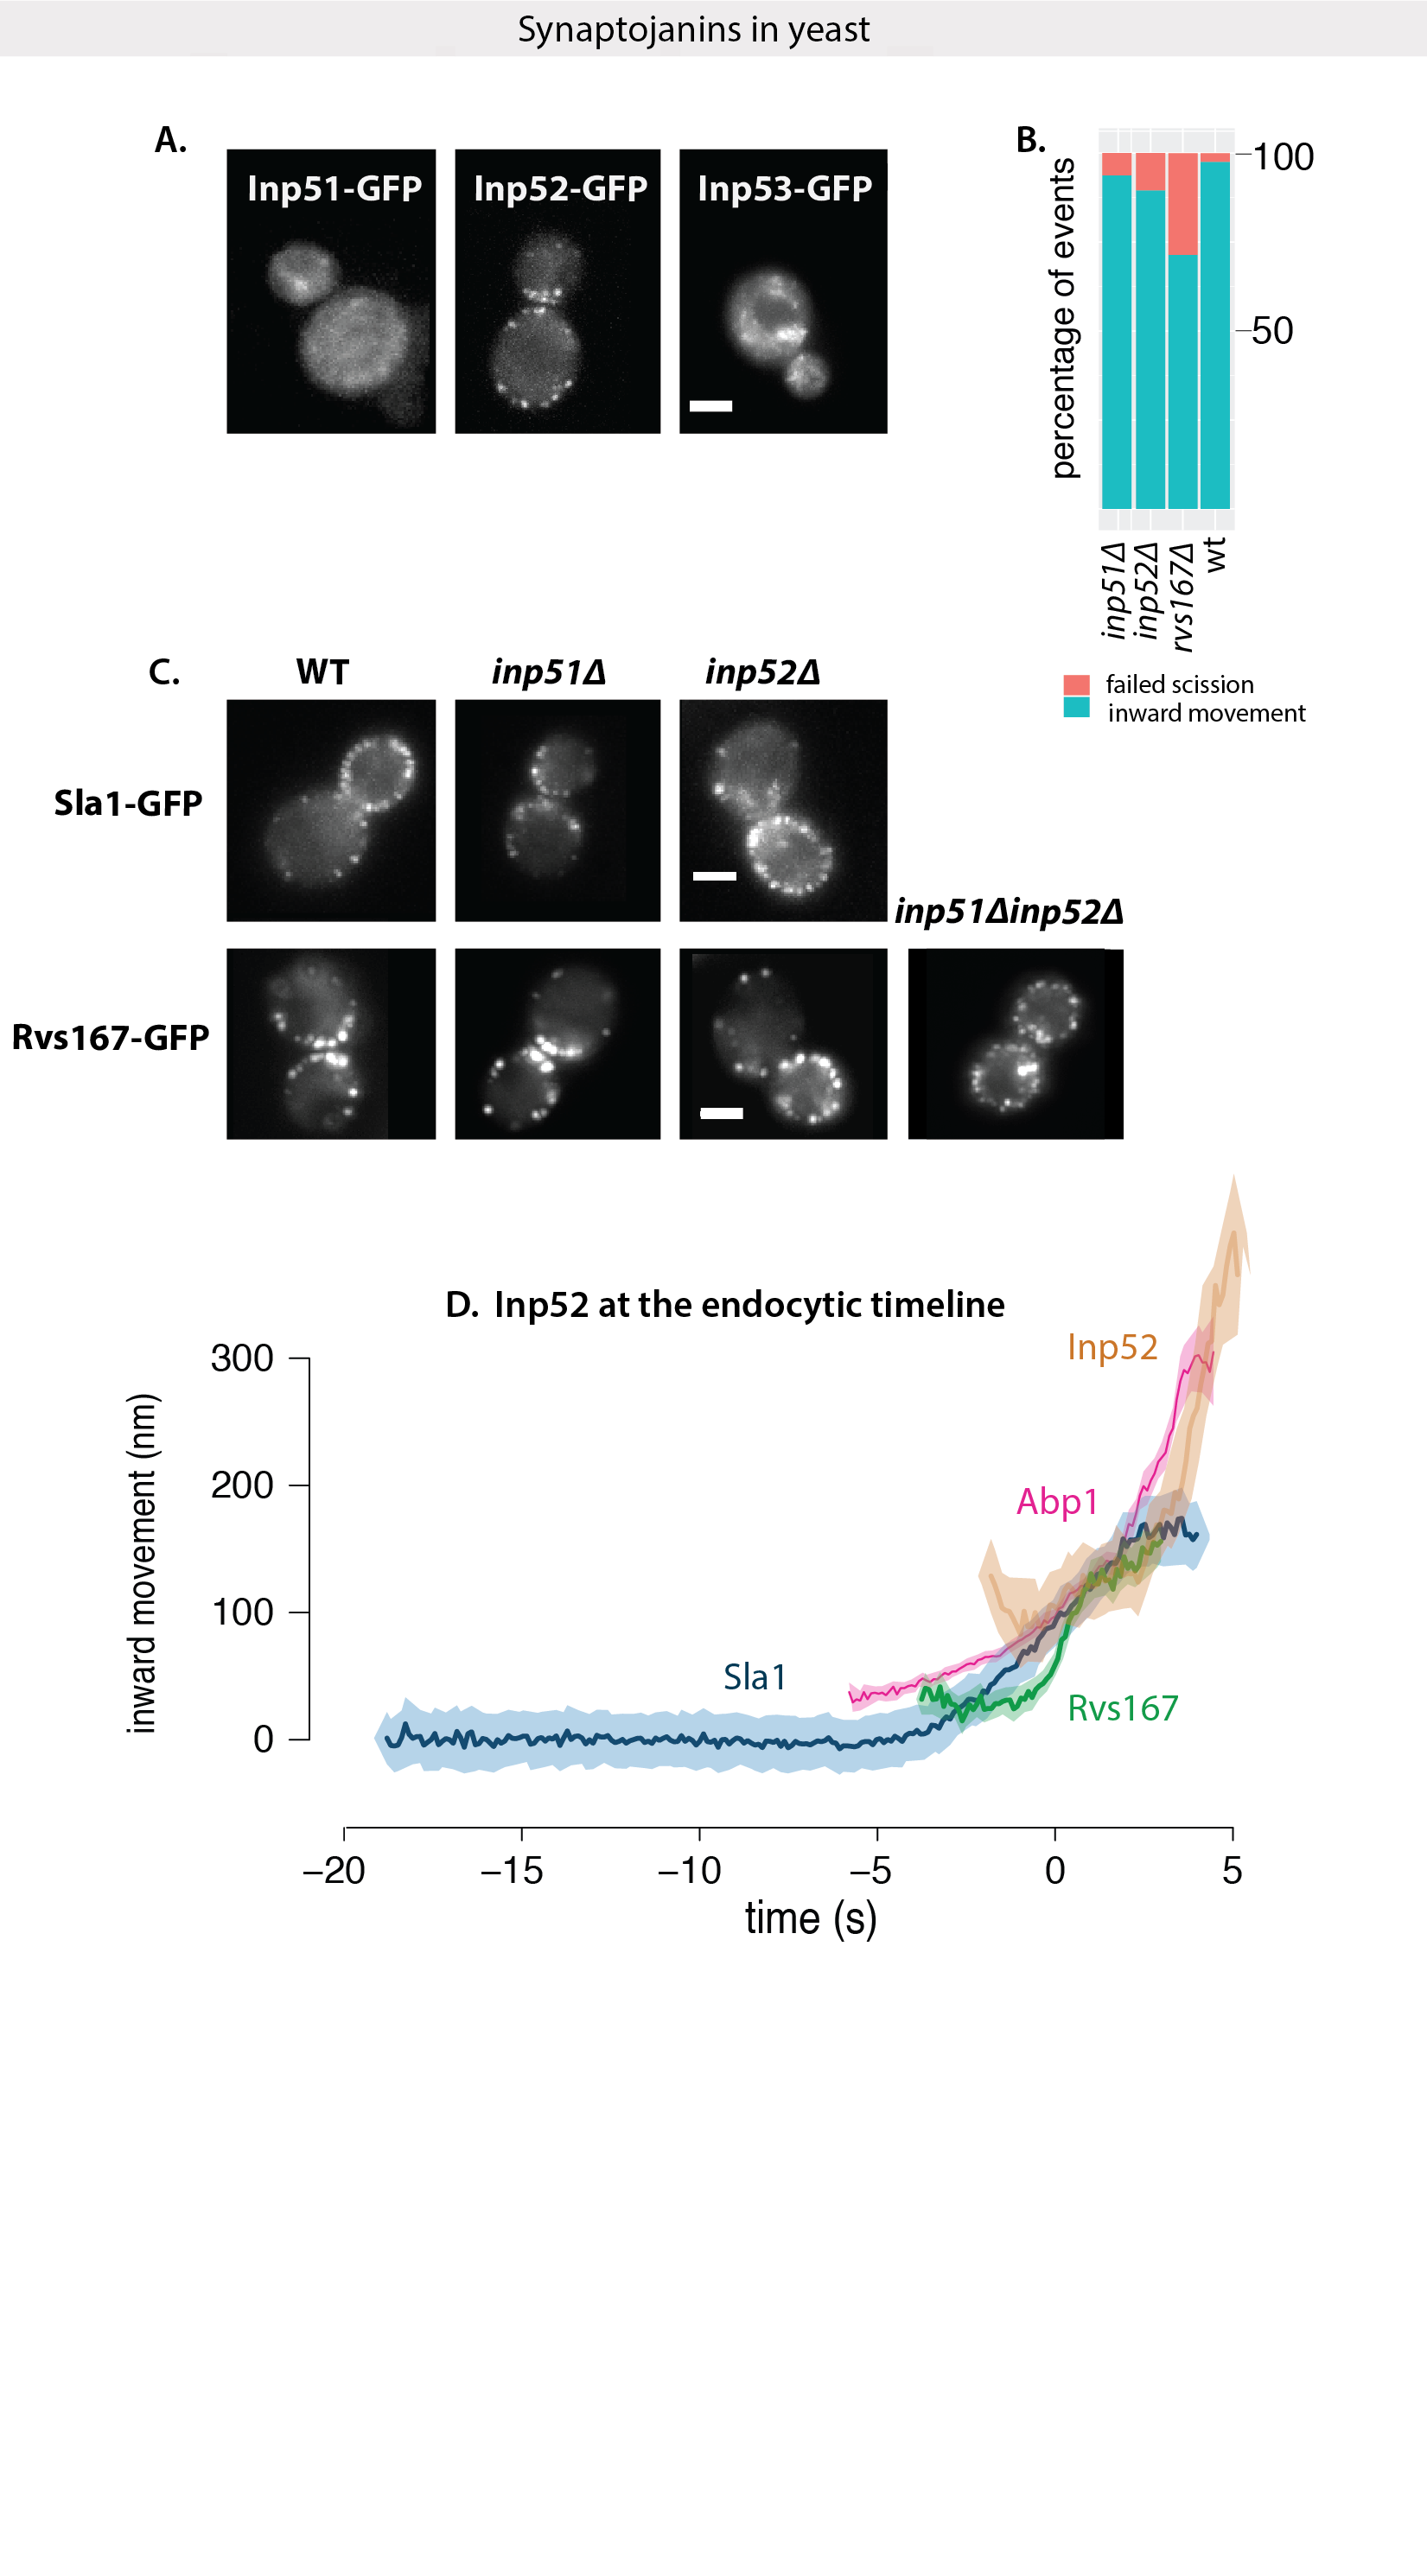
\includegraphics[width=19cm,height=19cm,keepaspectratio]{figures/results_final/inp}
			\caption[Synaptojanin-like proteins in yeast]
			{A: Maximum intensity projections of time-lapse images of cells expressing GFP-tagged Synaptojanin-like proteins Inp51, Inp52, and Inp53. Exposure rate 80ms.
			B: Failure rate of membrane scission, measured by quantifying number of retractions of Sla1 after membrane begins to move inwards, or by total lack of movement in WT, \textit{rvs167$\Delta$}, \textit{inp51$\Delta$} and \textit{inp52$\Delta$} strains.
			C: Sla1-GFP in WT,  \textit{inp51$\Delta$}  and  \textit{inp52$\Delta$} strains show similar plasma membrane localization. Rvs167-GFP in WT, \textit{inp51$\Delta$}, \textit{inp52$\Delta$} and \textit{inp51$\Delta$}\textit{inp52$\Delta$} strains. 
			D: Inp52-GFP in endocytic timeline in WT cells. Time=0 (s) corresponds to scission time.
			All scale bars =2um.
			\label{fig_inp}}
			\end{figure}
				

	\begin{figure}[H]
	\centering
	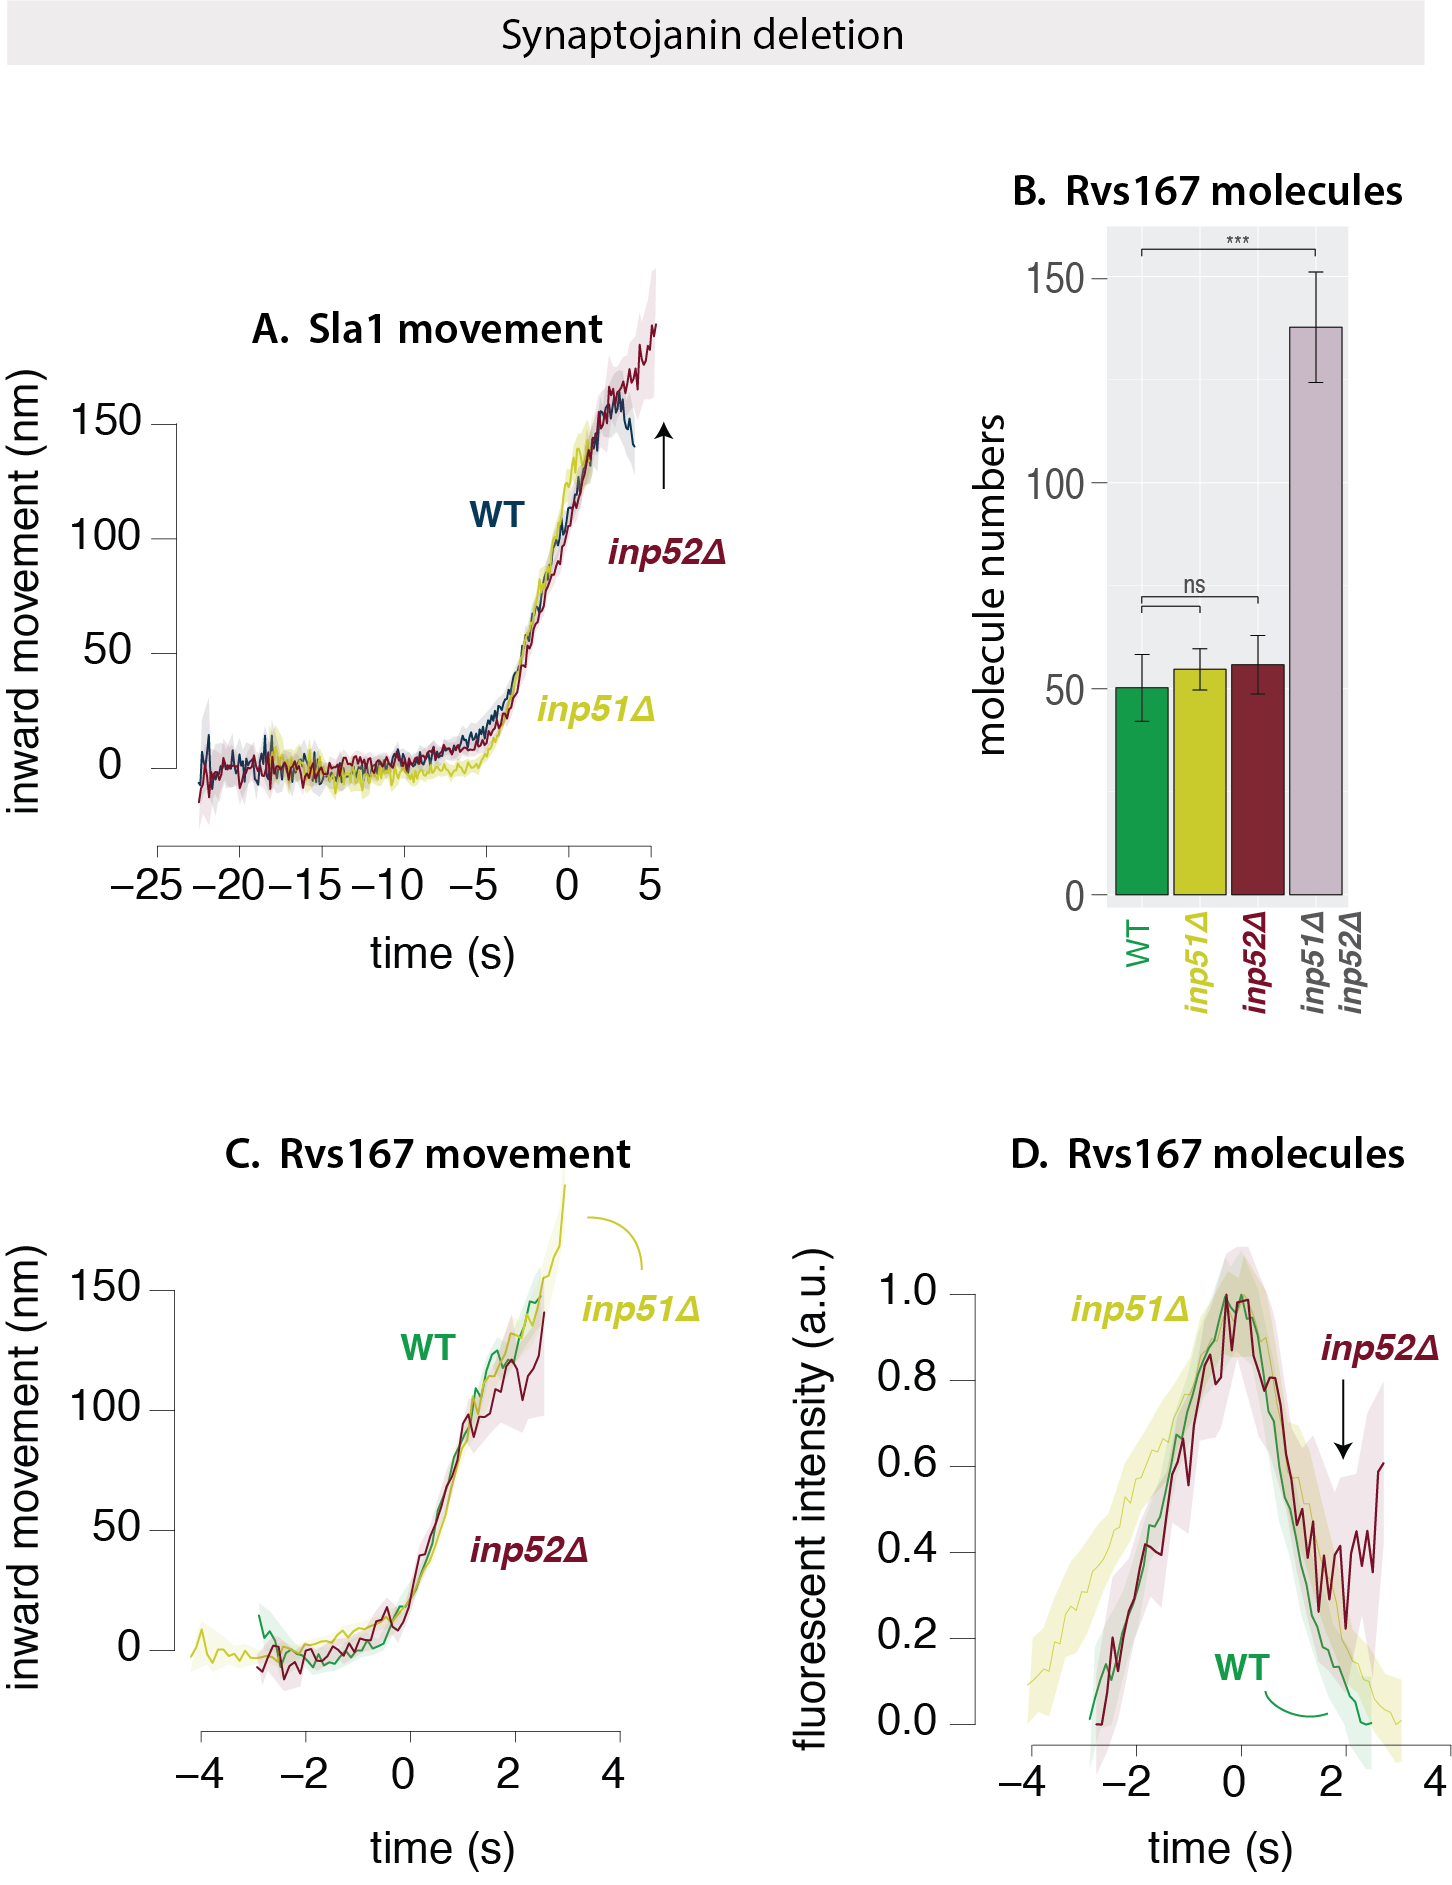
\includegraphics[width=19cm,height=19cm,keepaspectratio]{figures/results_final/inp_movement3}
	\caption[Synaptojanin deletion]
	{A: Movement of Sla1 in WT, Inp51del and Inp52del strains. 
		B: Median number of Rvs167 molecules recruited to endocytic sites in WT, \textit{inp52$\Delta$}, \textit{inp52$\Delta$ } and \textit{inp51$\Delta$inp52$\Delta$ } cells. P-values from two-sided z test,  * = p $\leq$ 0.05 , ** = p$\leq$ 0.01, *** = p $\leq$ 0.001.  
		C: Movement of Rvs167 in WT, \textit{inp51$\Delta$ } and \textit{inp52$\Delta$ } strains. 
		D: Normalized fluorescent intensity of averaged Rvs167 patches in WT, \textit{inp51$\Delta$ }, \textit{inp52$\Delta$ } cells.
		\label{fig_inpmov}}
\end{figure}

	\subparagraph{Rvs generates frictional forces on the membrane}
	Recent in-vitro experiments have proposed protein friction as a BAR-driven mechanism for membrane scission33. In this model, a BAR domain scaffold on a membrane tube forms a frictional barrier to lipid diffusion. Forces that pull on the membrane increase the frictional force exerted by the scaffold on the underlying membrane tube. This leads to membrane thinning in the region not covered by the BAR, since there is no lipid influx. In turn, this leads to increased membrane tension in this region. Eventually, membrane pores form in this portion of the tube, which break the tube, forming a vesicle. In-vivo, the forces pulling the membrane could be provided by molecular motors like myosins or actin polymerization.
This moΔpredicts that if more BAR proteins are added, and at a faster rate, to the membrane, frictional force would increase. If frictional force increases, scission would occur faster: that is, at shorter invagination lengths compared to a membrane with fewer BAR proteins. 

	\subsection{Membrane scission does not occur at shorter tube lengths when recruitment of Rvs is increased}
	
To test whether protein friction could effect membrane scission in yeast, I duplicated the Rvs167 and Rvs161 genes as described in Huber et al34. Gene duplication is performed in haploid cells to produce strains that have one (WT in haploids: 1xh) and two copies (2xh) of both Rvs161 and Rvs167 genes. These haploid strains are then mated to generate diploid strains that have four copies of Rvs167 and Rvs161 genes (4xd), two copies (WT in diploids: 2xd). Cells containing 1x copy of Rvs is generated by crossing rvs167Δstrain with an rvs161Δstrain (1xd). Compared to haploid strains expressing Rvs167-GFP, diploid strains appear to have more endocytic patches (Fig.2.10B). 

\cite{Dem} 
	

		\subparagraph]{Sla1 and Rvs in gene duplicated haploids:}

In Fig.2.8A, Sla1 movement in WT (1xh) and duplicated (2xh) haploids are presented. WT Sla1 is aligned so that time= 0 (s) corresponds to scission time. Sla1 for 2xh is shifted so that it moves inwards at the same time as WT. Both Sla1 centroids move inwards at the same rate, and to the same distance of 140nm. 

I measured the number of Rvs molecules recruited to endocytic sites in 1xh and 2xh strains. The maximum number of Rvs molecules recruited in the 2xh strain is 180, compared to 114 in WT (see TABLE.1, Fig.2.8): 1.6x more Rvs is recruited to endocytic sites in the gene duplicated strain. In Fig.2.8B, fluorescent intensity of Rvs167 in 1xh and 2xh cells are shown. Both Rvs167 fluorescent intensity plots are aligned so that time=0 (s) corresponds to their respective maxima. Rvs accumulation takes the same amount of time in 1xh as in 2xh: rate at which Rvs molecules is recruited to endocytic sites is 1.6x in Rvs duplicated cells (Fig.2.8B). 

Dynamics of Rvs disassembly are quite different. Fig.2.8B shows that disassembly is slowed by ~1.5 seconds in 2xh compared to 1xh cell. In the corresponding Rvs centroid movement traces (Fig.2.8C), instead of the sharp jump seen in WT, there is a delay in movement into the cytoplasm.

		
				\vspace{5mm}
				\begin{figure}[h]
				\centering
				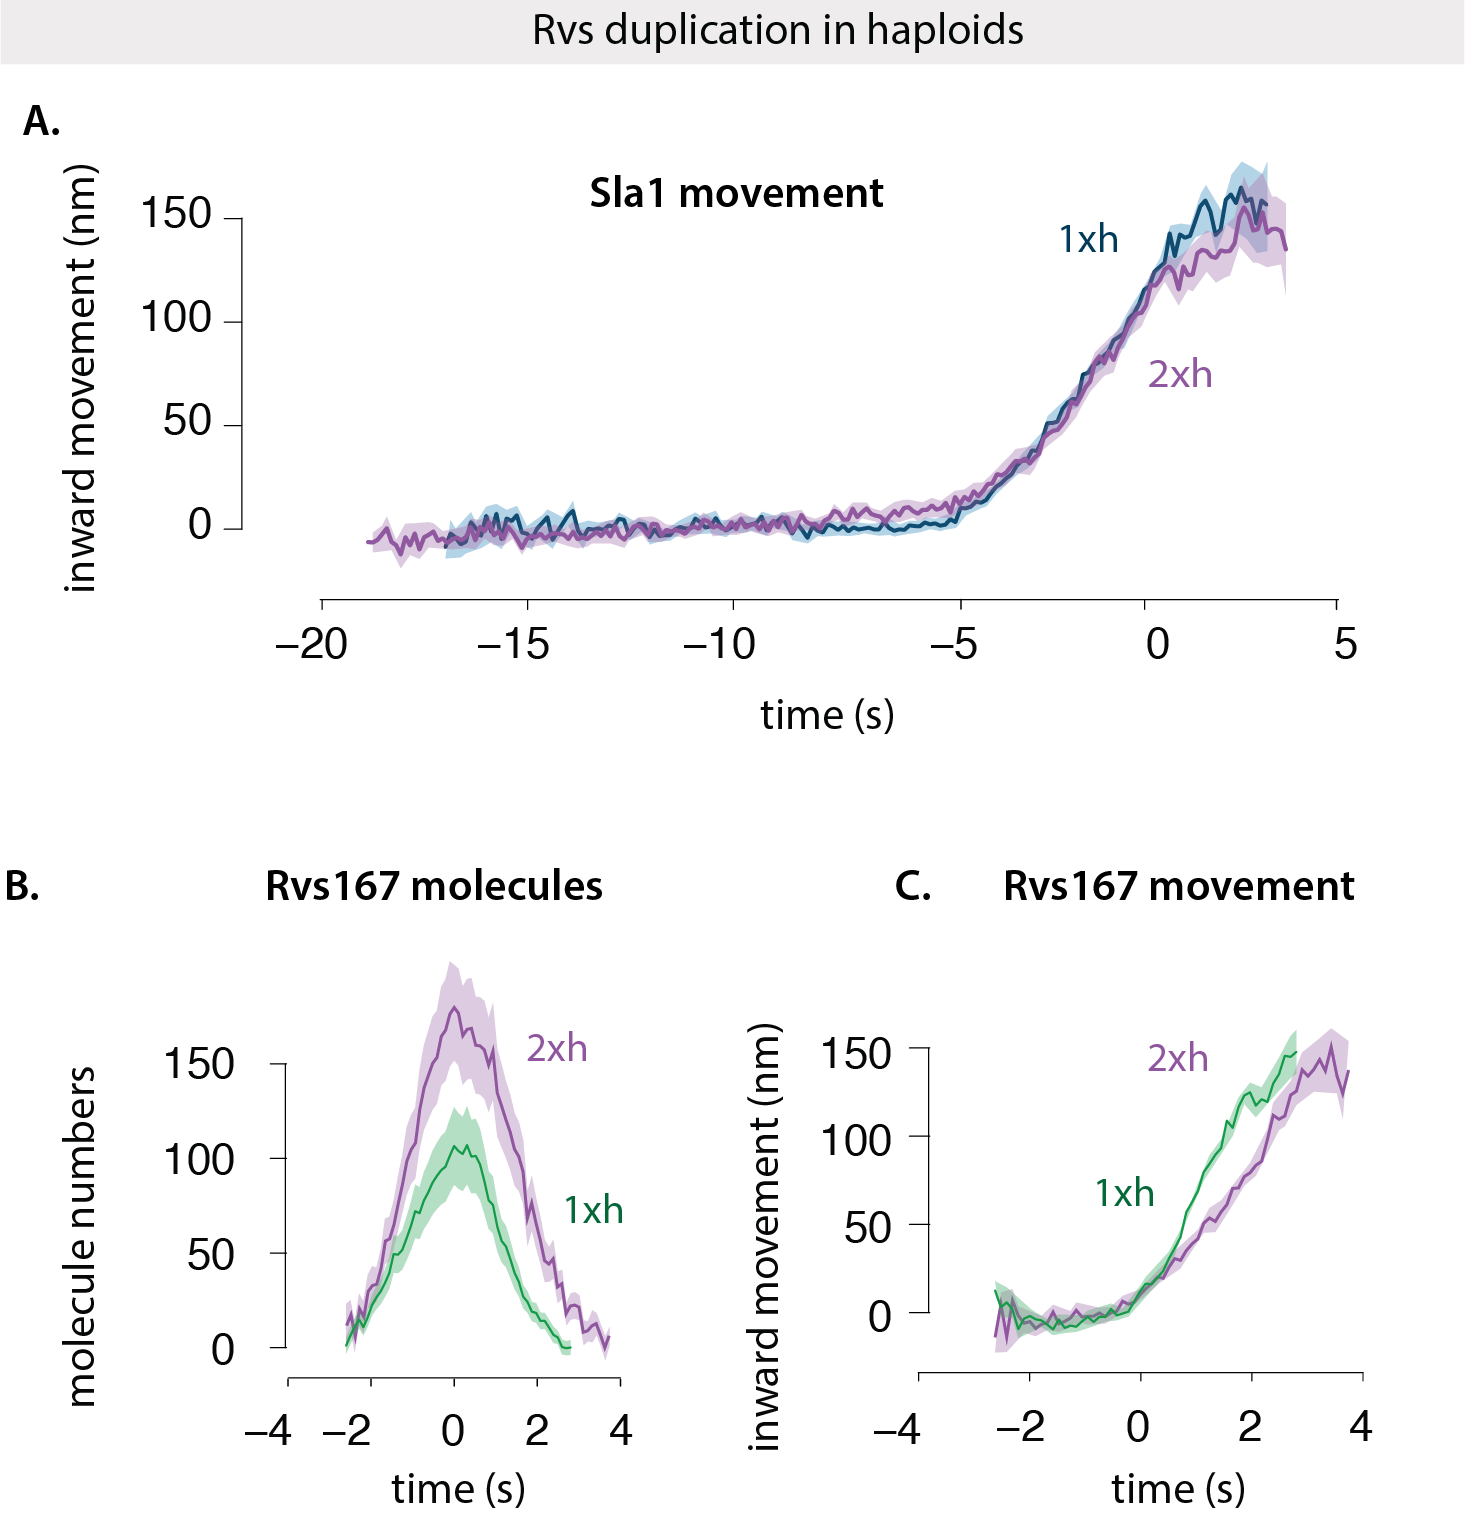
\includegraphics[width=13cm,height=13cm,keepaspectratio]{figures/results_final/rvs_haploid3}
				\caption[Overexpression of the Rvs complex in haploid cells]
					{A. Movement of Sla1 in WT (1x RVS) and gene-duplicated Rvs (2x RVS) cells. 1x RVS Sla1 is aligned so that time=0 (s) is scission time. 2x RVS Sla1 is shifted to move inwards at the same time.
					B. Recruitment of Rvs167 to sites in WT (1x Rvs)  and gene-duplicated Rvs (2x RVS) cells.1x RVS is aligned so that time = 0 (s) is scission time. 2x RVS Sla1 is shifted to move inwards at the same time.
					C.  Movement of Rvs167-GFP in WT (1x RVS) and gene-duplicated Rvs (2x RVS) cells. 1x RVS Rvs167 is aligned so that time=0 (s) is scission time. 2x RVS Rvs167 is shifted to move inwards at the same time.
			 \label{fig_rvshaploid}}

				\end{figure}
		
		\subparagraph]{Sla1 and Rvs in gene duplicated diploids:}

In diploid cells expressing 1 (1xd), 2 (2xd), and 4 (4xd) copies of Rvs, Sla1 movement, Rvs dynamics, and recruitment numbers are compared. 
In Fig.2.9A, Sla1 in the three cell types are shown. In all cases time=0 (s) corresponds to scission time. Sla1 movement is the same in 4xd and 2xd cells: they move at the same rate, and to the same lengths of about 140nm. In 1xd strain, Sla1 movement rate is the same till about 110nm, and is then slightly reduced. Sla1 movement in 1xd suggests that vesicle scission occurs at invagination lengths about 10nm shorter than that in 2xd and 4xd. 

Rvs167 movement and fluorescent intensities are shown in Fig.2.9 B,C. 
Magnitude of inward movement of the Rvs is similar for the 4xd, 2xd and 1xd. In the 1x strain, however, the centroid disappears immediately after scission, suggesting that there is reduced Rvs at the base of the newly formed vesicle compared to the 2xd and 4xd.

Recruitment dynamics of Rvs in all three are different: in the 4xd strain, Rvs is recruited at a rate of about 51 molecules/second, which is reduced to 27.5 molec./sec. for 2xd and 13.6 molec./sec. for the 1xd. Recruitment of Rvs is not directly proportionate to gene copy number: maximum number of Rvs recruited increases from 101 from in the 2x Rvs strain to 143 in the 4x strain (see TABLE1). In the 1x Rvs strain, 80 molecules of Rvs are recruited before scission occurs. In order to determine whether this is a reflection on protein availability or if something else limits recruitment of Rvs, I roughly quantified the cytoplasmic intensity of Rvs167-GFP in the respective strains, and scaled them to 2xd to obtain a ratio of cytoplasmic intensity compared to the WT. The number of molecules recruited to endocytic sites scales with the amount of protein in the cytoplasm (see methods).  




		\subparagraph]{	Abp1 amounts in gene duplicated diploids:}
		I measured the amount of Abp1 at endocytic sites in 4xd, 2xd, and 1xd diploid cells. Abp1 numbers provided in Fig.2.10B are quantified in cells containing Rvs167-GFP and Abp1-mCherry.  Abp1-mCherry signal is then scaled to Nuf2-mCherry, similar to quantification method in Picco et al. that uses GFP instead of mCherry. Fig2.10B shows that even though the number of Rvs molecules recruited varies depending on number of Rvs gene copies, the same amount of Abp1 is recruited to endocytic sites in all three cases. In the Abp1 quantification in this case, only one allele of Abp1 is tagged with mCherry. The total amount of Abp1 is double the numbers reported here. 

Rvs gene duplication data suggests that even if Rvs is recruited up to 1.6x faster than in WT cells, membrane invaginations do not change in length. That the same amount of Abp1 is recruited irrespective of amount of Rvs suggests that the system is sensitive to amount of Abp1 rather than Rvs. Scission time is therefore likely to be triggered by the amount of force generated by the actin network. 



\newpage
						\begin{figure}[H]
						\centering
						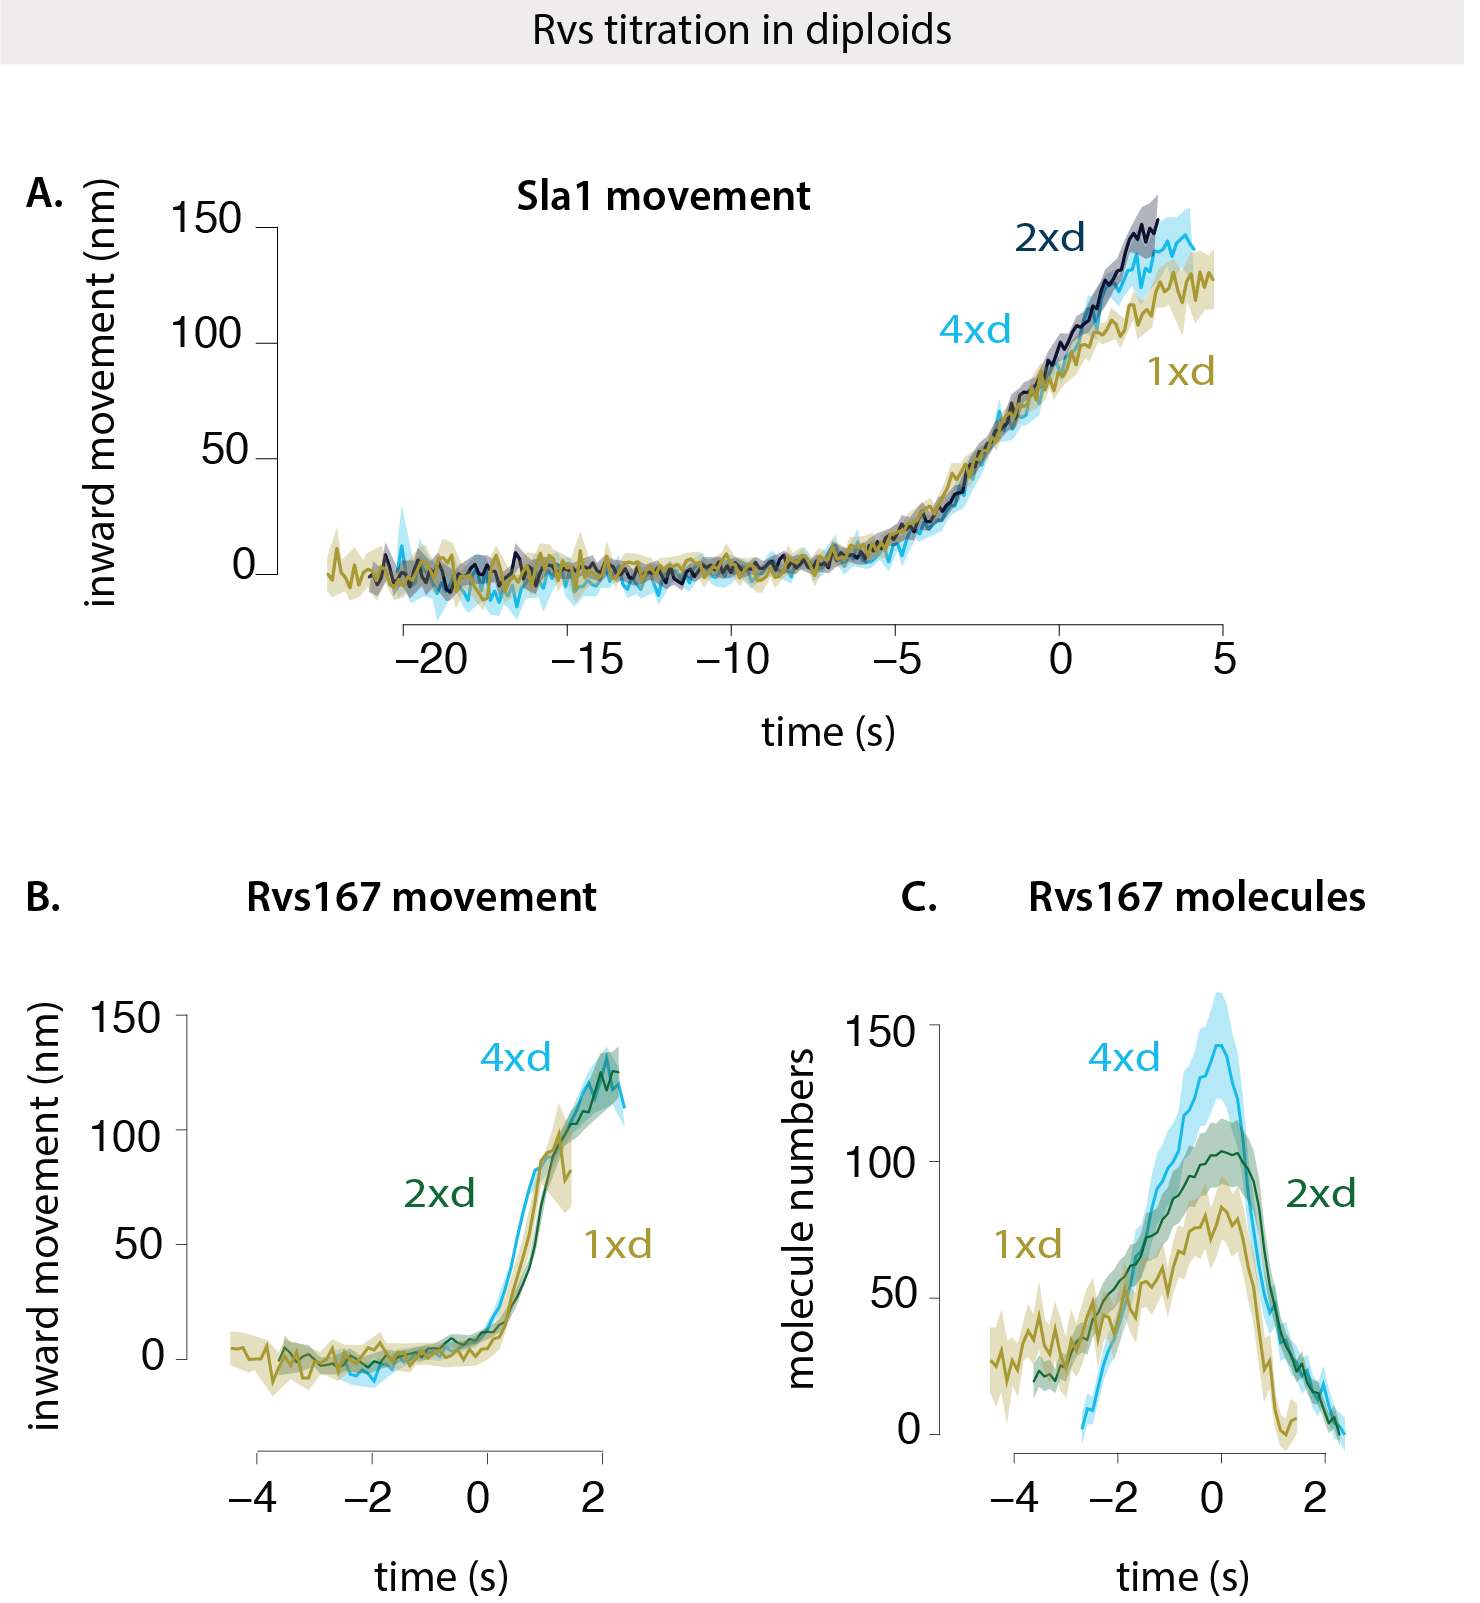
\includegraphics[width=22cm,height=22cm,keepaspectratio]{figures/results_final/protein_friction4}
						\caption[Dynamics of endocytosis in diploid strains with gene duplicated Rvs]
						{A. Movement of Sla1 in WT (1x RVS) and gene-duplicated Rvs (2x RVS) cells. 1x RVS Sla1 is aligned so that time=0 (s) is scission time. 2x RVS Sla1 is shifted to move inwards at the same time.
						B. Recruitment of Rvs167 to sites in WT (1x Rvs)  and gene-duplicated Rvs (2x RVS) cells.1x RVS is aligned so that time = 0 (s) is scission time. 2x RVS Sla1 is shifted to move inwards at the same time.
						C.  Movement of Rvs167-GFP in WT (1x RVS) and gene-duplicated Rvs (2x RVS) cells. 1x RVS Rvs167 is aligned so that time=0 (s) is scission time. 2x RVS Rvs167 is shifted to move inwards at the same time.
						\label{fig_rvsdiploid}}
						\end{figure}
				
						\begin{figure}[H]
	\centering
	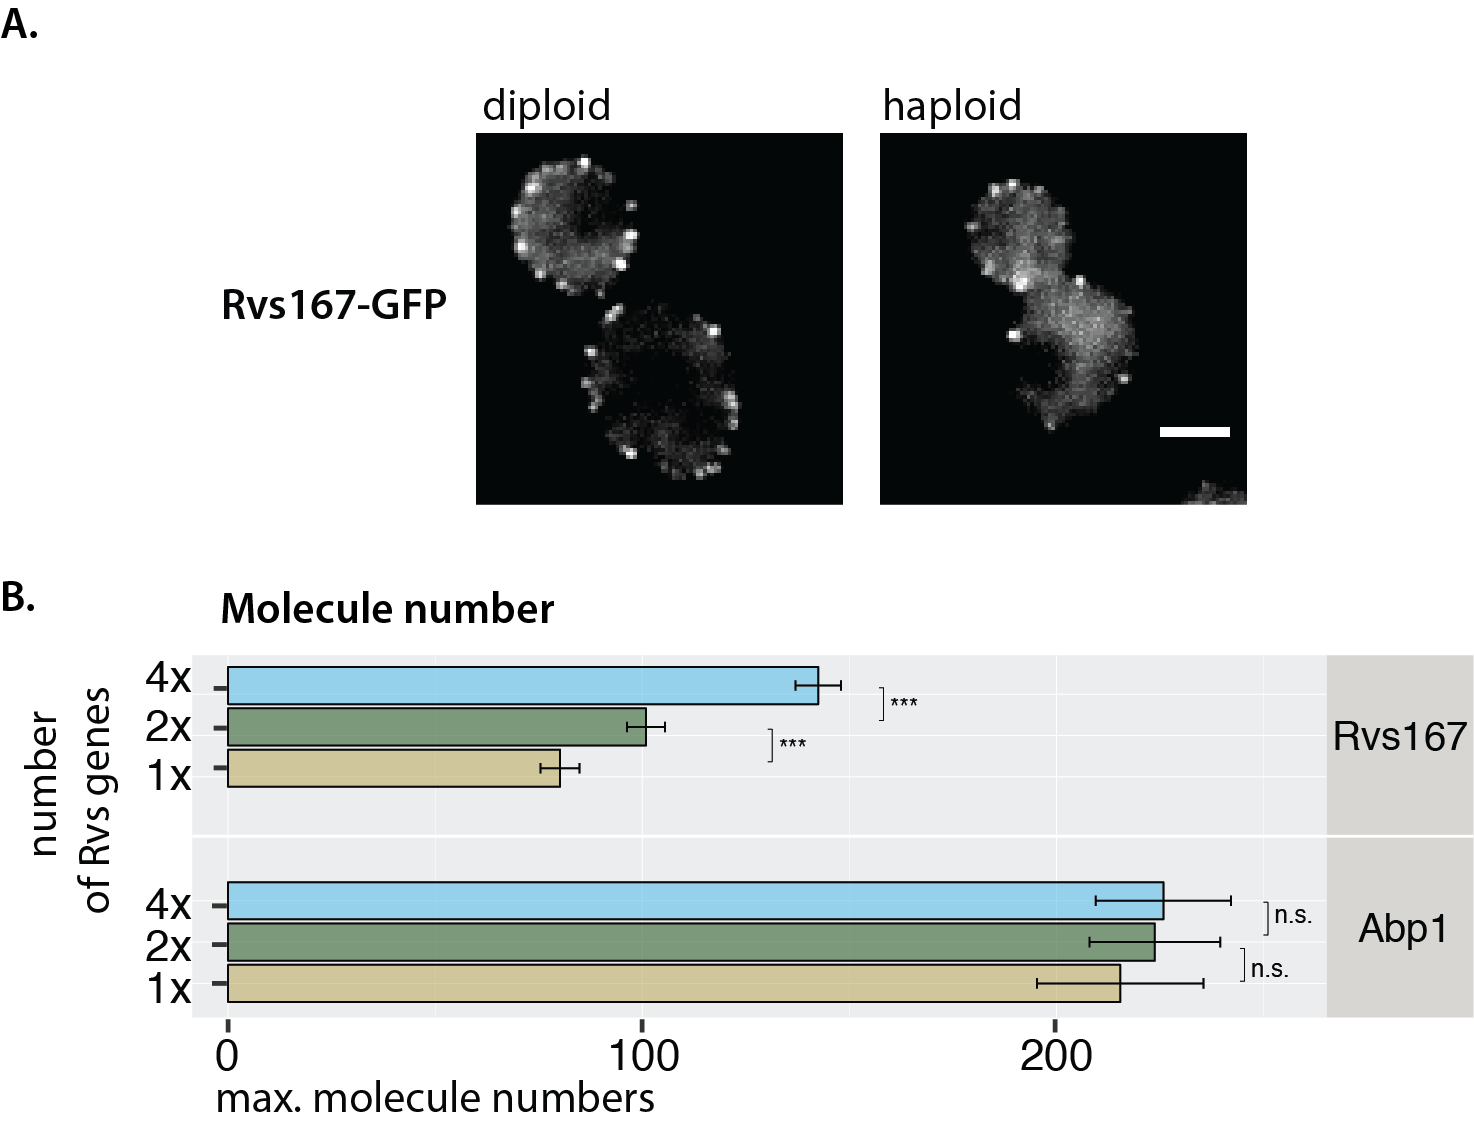
\includegraphics[width=22cm,height=22cm,keepaspectratio]{figures/results_final/protein_frictionB}
	\caption[Dynamics of endocytosis in diploid strains with gene duplicated Rvs]
	{A. Movement of Sla1 in WT (1x RVS) and gene-duplicated Rvs (2x RVS) cells. 1x RVS Sla1 is aligned so that time=0 (s) is scission time. 2x RVS Sla1 is shifted to move inwards at the same time.
		B. Recruitment of Rvs167 to sites in WT (1x Rvs)  and gene-duplicated Rvs (2x RVS) cells.1x RVS is aligned so that time = 0 (s) is scission time. 2x RVS Sla1 is shifted to move inwards at the same time.
		C.  Movement of Rvs167-GFP in WT (1x RVS) and gene-duplicated Rvs (2x RVS) cells. 1x RVS Rvs167 is aligned so that time=0 (s) is scission time. 2x RVS Rvs167 is shifted to move inwards at the same time.
		\label{fig_rvsdiploid}}
\end{figure}


\newpage
	\subparagraph{BAR domains as membrane scaffolds}
	As mentioned in section R.1, the capacity for BAR domains to oligomerize and tubulate liposomes has proposed membrane scaffolding as a possible function in vivo. As membrane scaffolds, they would impose their own curvature on the underlying membrane and stabilize this shape. There are some requirements for a protein complex to act as a scaffold35:
	1. it must have a defined membrane interface\\
	2. it must have an intrinsic curvature\\
	3. it must present be rigid in structure, and\\
	4. membrane binding surface must be large enough to induce curvature\\

BAR domains present a curved shape as membrane interacting surface13,36,37, and have the capacity to oligomerize into large assemblies on tubes9,38,39. It has also been shown that the central BAR region is rigid and required for tubulation, both in-vivo and of liposomes40. BAR domains therefore meet all of these requirements. 
	
It has been shown that BAR domains can prevent membrane scission by scaffolding the membrane, allowing formation of stable tubular structures and preventing vesiculation of these structures5,12 . In simulations, adding BAR domains to an invaginating tube removes membrane shape instabilities. Actin forces, membrane rigidity and tension, and turgor pressure result in a wide invagination tip and shrinking tubular region that result in membrane shape instability and therefore scission. Adding curved BAR domains that have a preferred radius of curvature results in stabilization of the membrane shape and prevents scission34.

	\subsection{Coat movement is influenced by recruitment of BAR domain }
As observed in the previous section R2.3, Sla1 movement is decreased by decreased recruitment of Rvs, although adding excess protein does not influence it. In BAR cells Sla1 movement is reduced from WT to close to that of rvs167Δ. However, Rvs recruitment is also decreased. Reduced coat movement therefore could result from loss of the SH3 domain, or from reduced Rvs recruitment. To test this, I duplicated as described before, the BAR domain alone in haploid yeast cells. This results in two copies of the BAR domain (2xBAR). I then compared Sla1 and Rvs  in 2xBAR against BAR (1xBAR), WT Rvs (1xh), duplicated Rvs (2xh), and rvs167del.

I compared recruitment of Rvs in the different cells. As shown in Fig.2.11C, 1x BAR is recruited at low copy numbers compared to WT . Maximum molecules recruited is 57 +/- 9.9, about 50\% that of WT. Duplication of the BAR domain in 2x BAR increases this recruitment to 90.58 +/- 9.6. Compared to WT, recruitment of BAR domains increases to 62%. 

Sla1 moves inwards at a rate of about 26nm/s. While duplication of the full-length Rvs genes does not change the rate of inward movement of Sla1, total rate of inward movement is reduced to 13.3nm/s in 1x BAR case. This rate increases to about 18nm/s in the 2x BAR case. Adding BAR domain increases the speed of inward movement, as well as depth to which Sla1 moves. Sla1 centroid in rvs167 deleted cells shows a movement similar to 1x BAR case. Rvs167 dynamics similar to WT can also be recapitulated by adding increasing amounts of Rvs167 (Fig.2.11B,C).

This shows that shallow invaginations of the rvs167Δ can be rescued by recruiting only BAR domains of Rvs167.


		\begin{figure}[H]
		\centering
		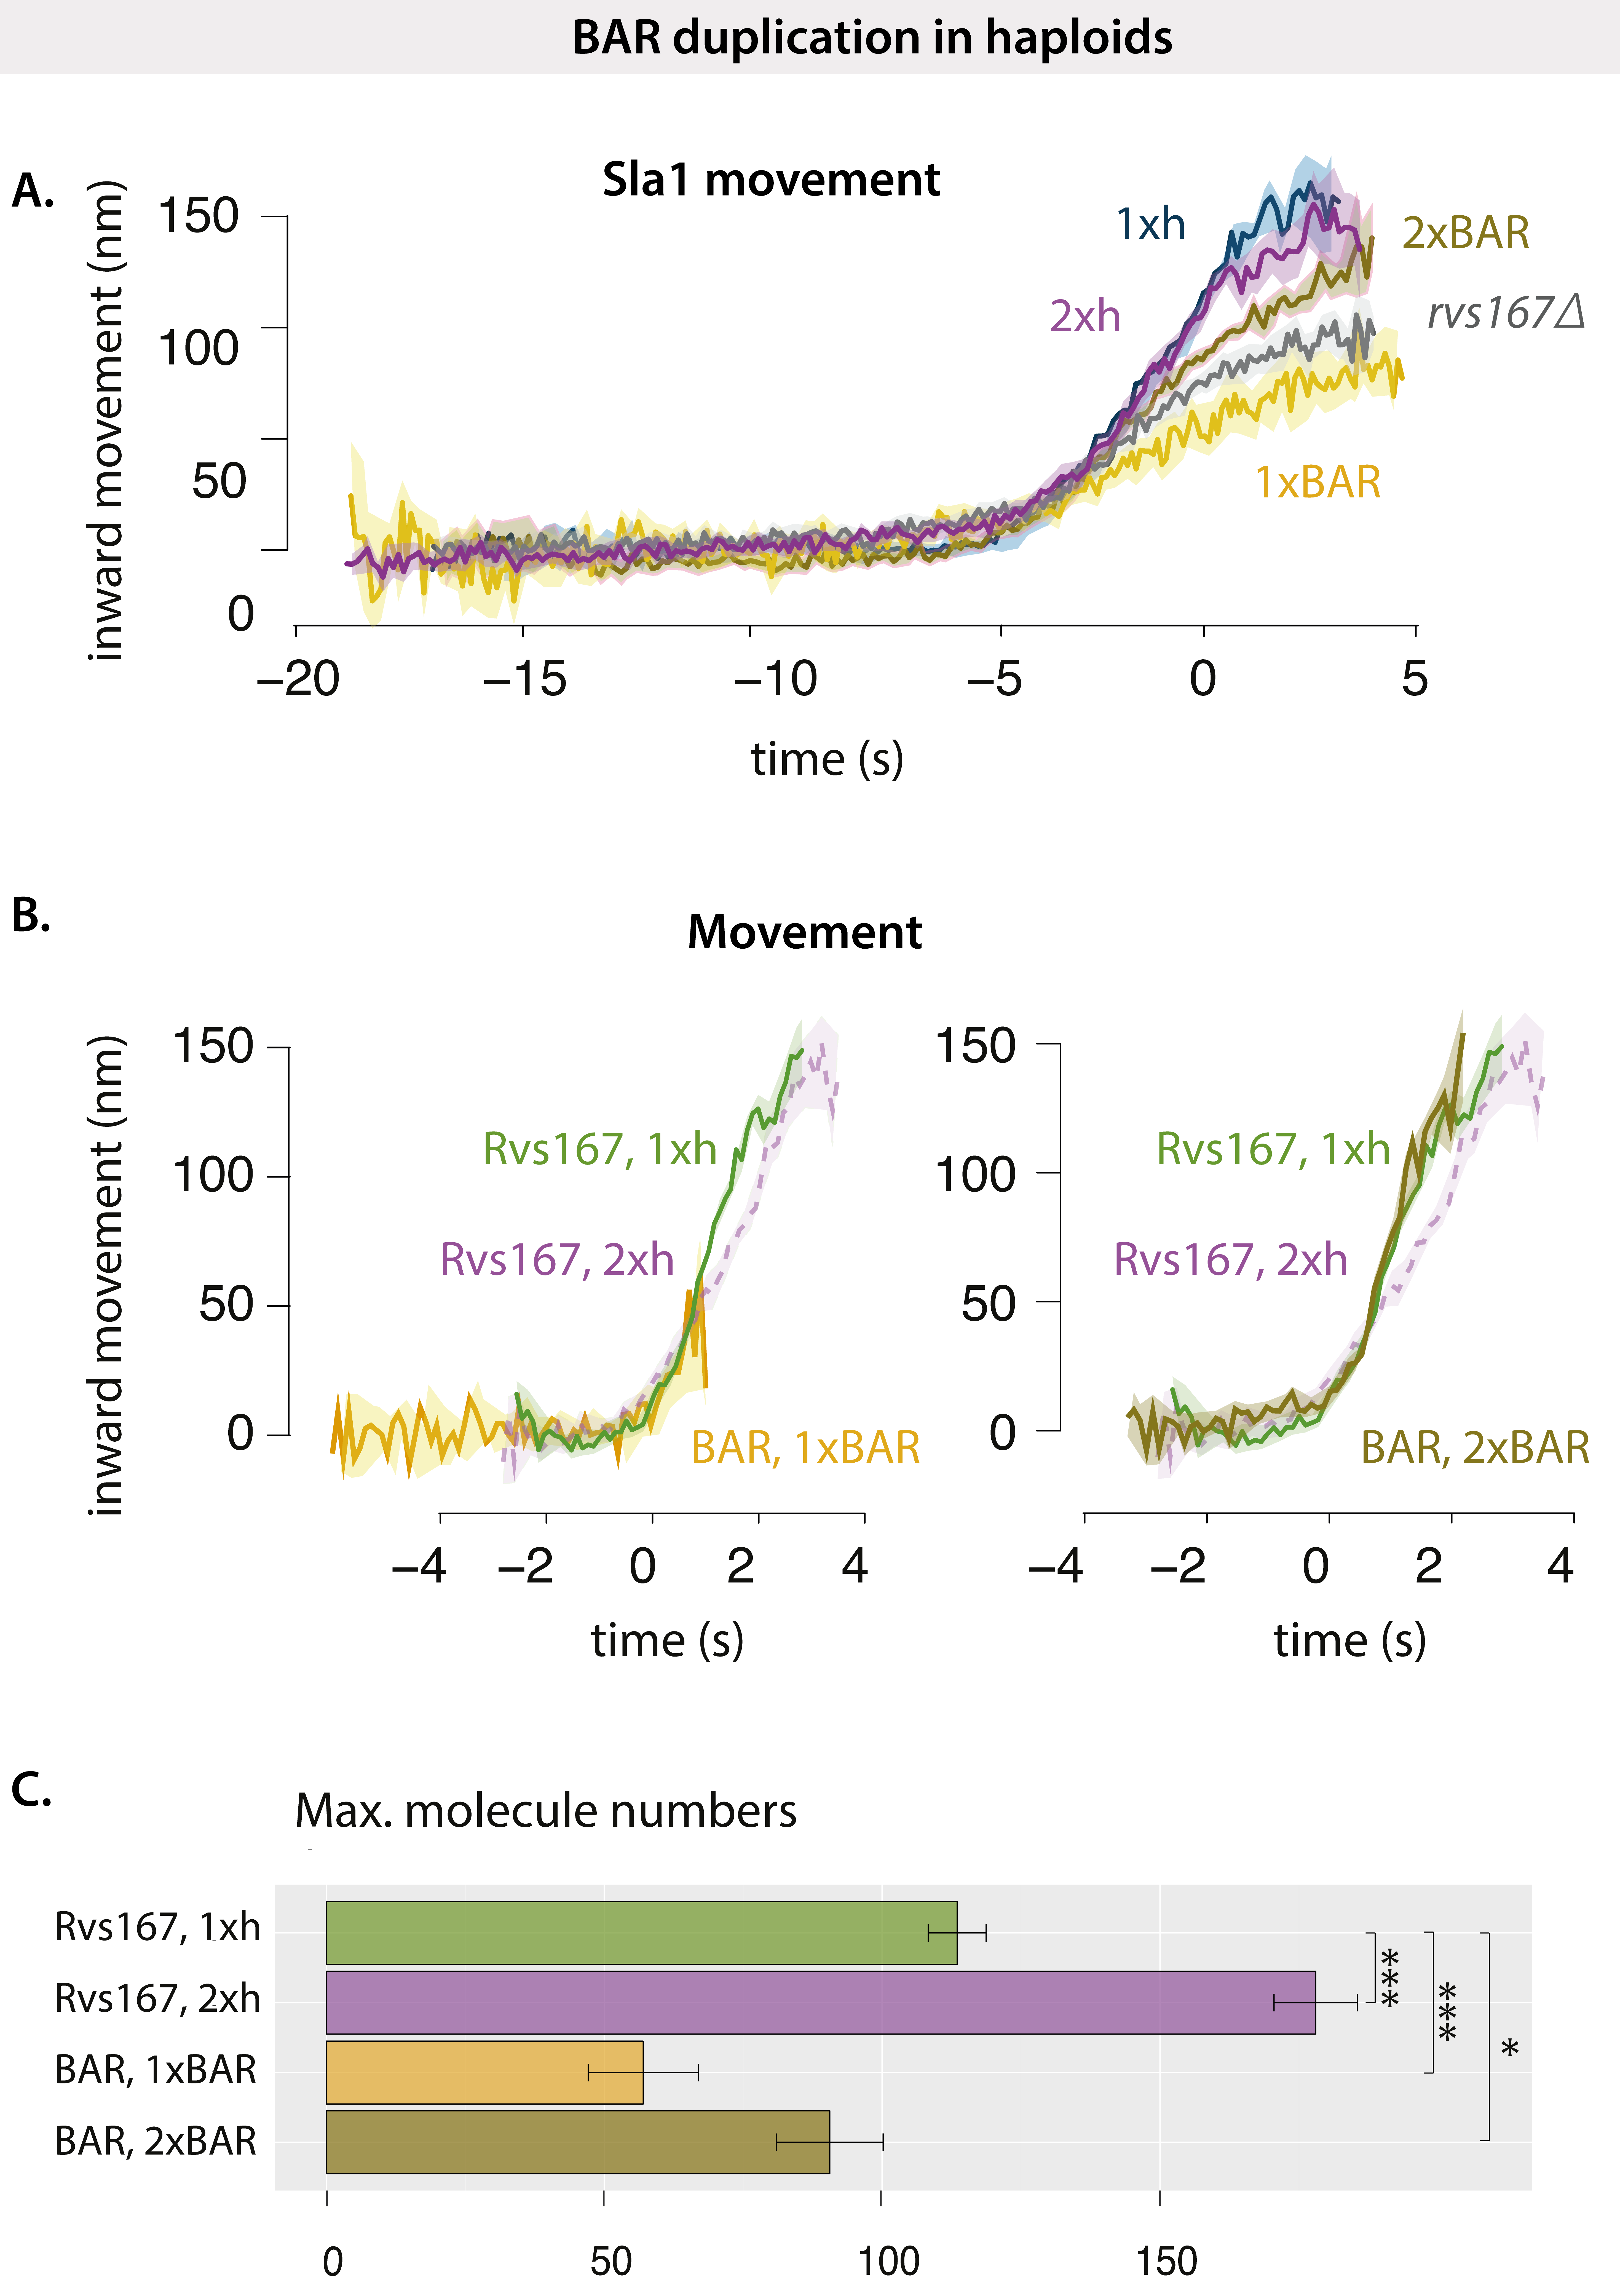
\includegraphics[width=25cm,height=25 cm,keepaspectratio]{figures/results_final/scaffolding_overlaid3}
		\caption [Progression of invagination with increasing BAR recruitment]
		{A:Averaged centroid movement of Sla1 in strains expressing varying gene copy numbers of Rvs complex, and \textit{rvs167$\Delta$}. 1x Rvs=WT expression, 2x = Rvs167 and Rvs161 genes are duplicated. 1xBAR=Rvs167 without the SH3 domain, 2xBAR=Rvs167 without the SH3 domain is duplicated. Averages are aligned in time so that time=0 (s) for WT Sla1-GFP corresponds to scission time. Other averages have been shifted to move inwards at the same time as the WT.
		B: Averaged centroid movement of Rvs167-GFP in 1x RVS, 2xRVS, 1xBAR, 2XBAR strains.
		C:  }
		\label{fig_scaffold}
		\end{figure}


	\subparagraph{Rvs as a scaffold against turgor pressure} 
	
Pressure, membrane tension, and rigidity influence the shape of membrane invaginations. In yeast, a high turgor pressure of 0.6 - 0.8 MPa pushes the plasma membrane against the cell wall. This pressure is opposed by the rigid cell wall, and the endocytic machinery must exert forces to bend and pull the plasma membrane away from the cell wall into the cytoplasm. Forces from actin polymerization are hence necessary to overcome this resistance to membrane invagination. In serge et al., simulations show that membrane tension has a negligible influence on forces required to pull the membrane. Shape of the membrane is dominated by membrane rigidity and turgor pressure. Membrane rigidity, which comes from the properties of the lipids and proteins embedded in it shapes the shape of the top of the invagination that is pulled up. Turgor pressure pushes inwards the membrane neck, constricting it. 

Turgor pressure can be controlled by osmoregulating agents like sorbitol. Sorbitol treatment causes cells to expel water and increase the internal concentration of osmolytes to match that of the environment. When the cell expels water, they shrink in size, resulting in a brief decrease of turgor pressure. Loss of turgor pressure is compensated by Gpd1, which increases glycerol production in cells, and increases turgor pressure within 10 minutes of sorbitol treatment.

In fission yeast S.pombe, treatment with sorbitol shortens the time between arrival of the coat protein Sla1 and actin-binding protein App1, but does not affect the inward movement of the coat42. Sorbitol rescues the invagination defect of partially blocking actin with low doses of LatA. At 0.2M sorbitol, 90\% of Sla1 patches in these cells move inwards for 50nm instead of 300nm, but retract back to the plasma membrane. 

Some WASP/Myosin mutations can be rescued by reducing turgor pressure. Deletion of myosin results in failure to invaginate, and this can be rescued up to 70\% when treated with 0.2 M Sorbitol. Loss of Fimbrin, which bundles actin filaments, and is also necessary for membrane invagination, can also be rescued by sorbitol.  These experiments show that some defects in the force generation system can be compensated by lowering turgor pressure.  Since sorbitol decreases the amount of time between App1 arrival and movement, reducing turgor pressure likely lowers the threshold force required to pull the membrane in the early stages of invagination. Consistent with this, simulations of Serge et al., show that the force requirement for membrane invagination is highest in the beginning of the invagination process. 

An extension of the scaffold hypothesis for Rvs is that it protects the membrane tube against the high turgor pressure inside yeast cells. Reducing turgor pressure could then remove the requirement for Rvs scaffolding.

	\subsection{Requirement for Rvs is unchanged by membrane tension}
	In order to test if the role of the Rvs scaffold is to counter the membrane constricting effect of turgor pressure, I studied Sla1 and Rvs in WT and rvs167Δcells treated with 0.2M sorbitol. At higher concentrations of sorbitol, cells shrivel and do not recover from turgor pressure loss42.

In Fig.2.12, Sla1 movement in WT and rvs167 Δcells with and without sorbitol is shown. WT Sla1 is aligned so that time=0 (s) corresponds to scission time. The other three centroid movements are shifted so that they move inwards at the same time as the WT. WT cells treated with sorbitol do not show any change in inward movement of Sla1. Both centroids move to the same lengths of 140nm at the same rate, consistent with S.pombe data from Basu et al. In rvs167Δcells, Sla1 moves to about 80nm. In rvs167Δcells treated with sorbitol, there is no difference in the movement. Both Sla1 centroids move at the same rate, and to the similar invagination lengths.

This shows that the Rvs scaffold does not serve to counter turgor pressure.  

	\begin{figure}[H]
	\centering
	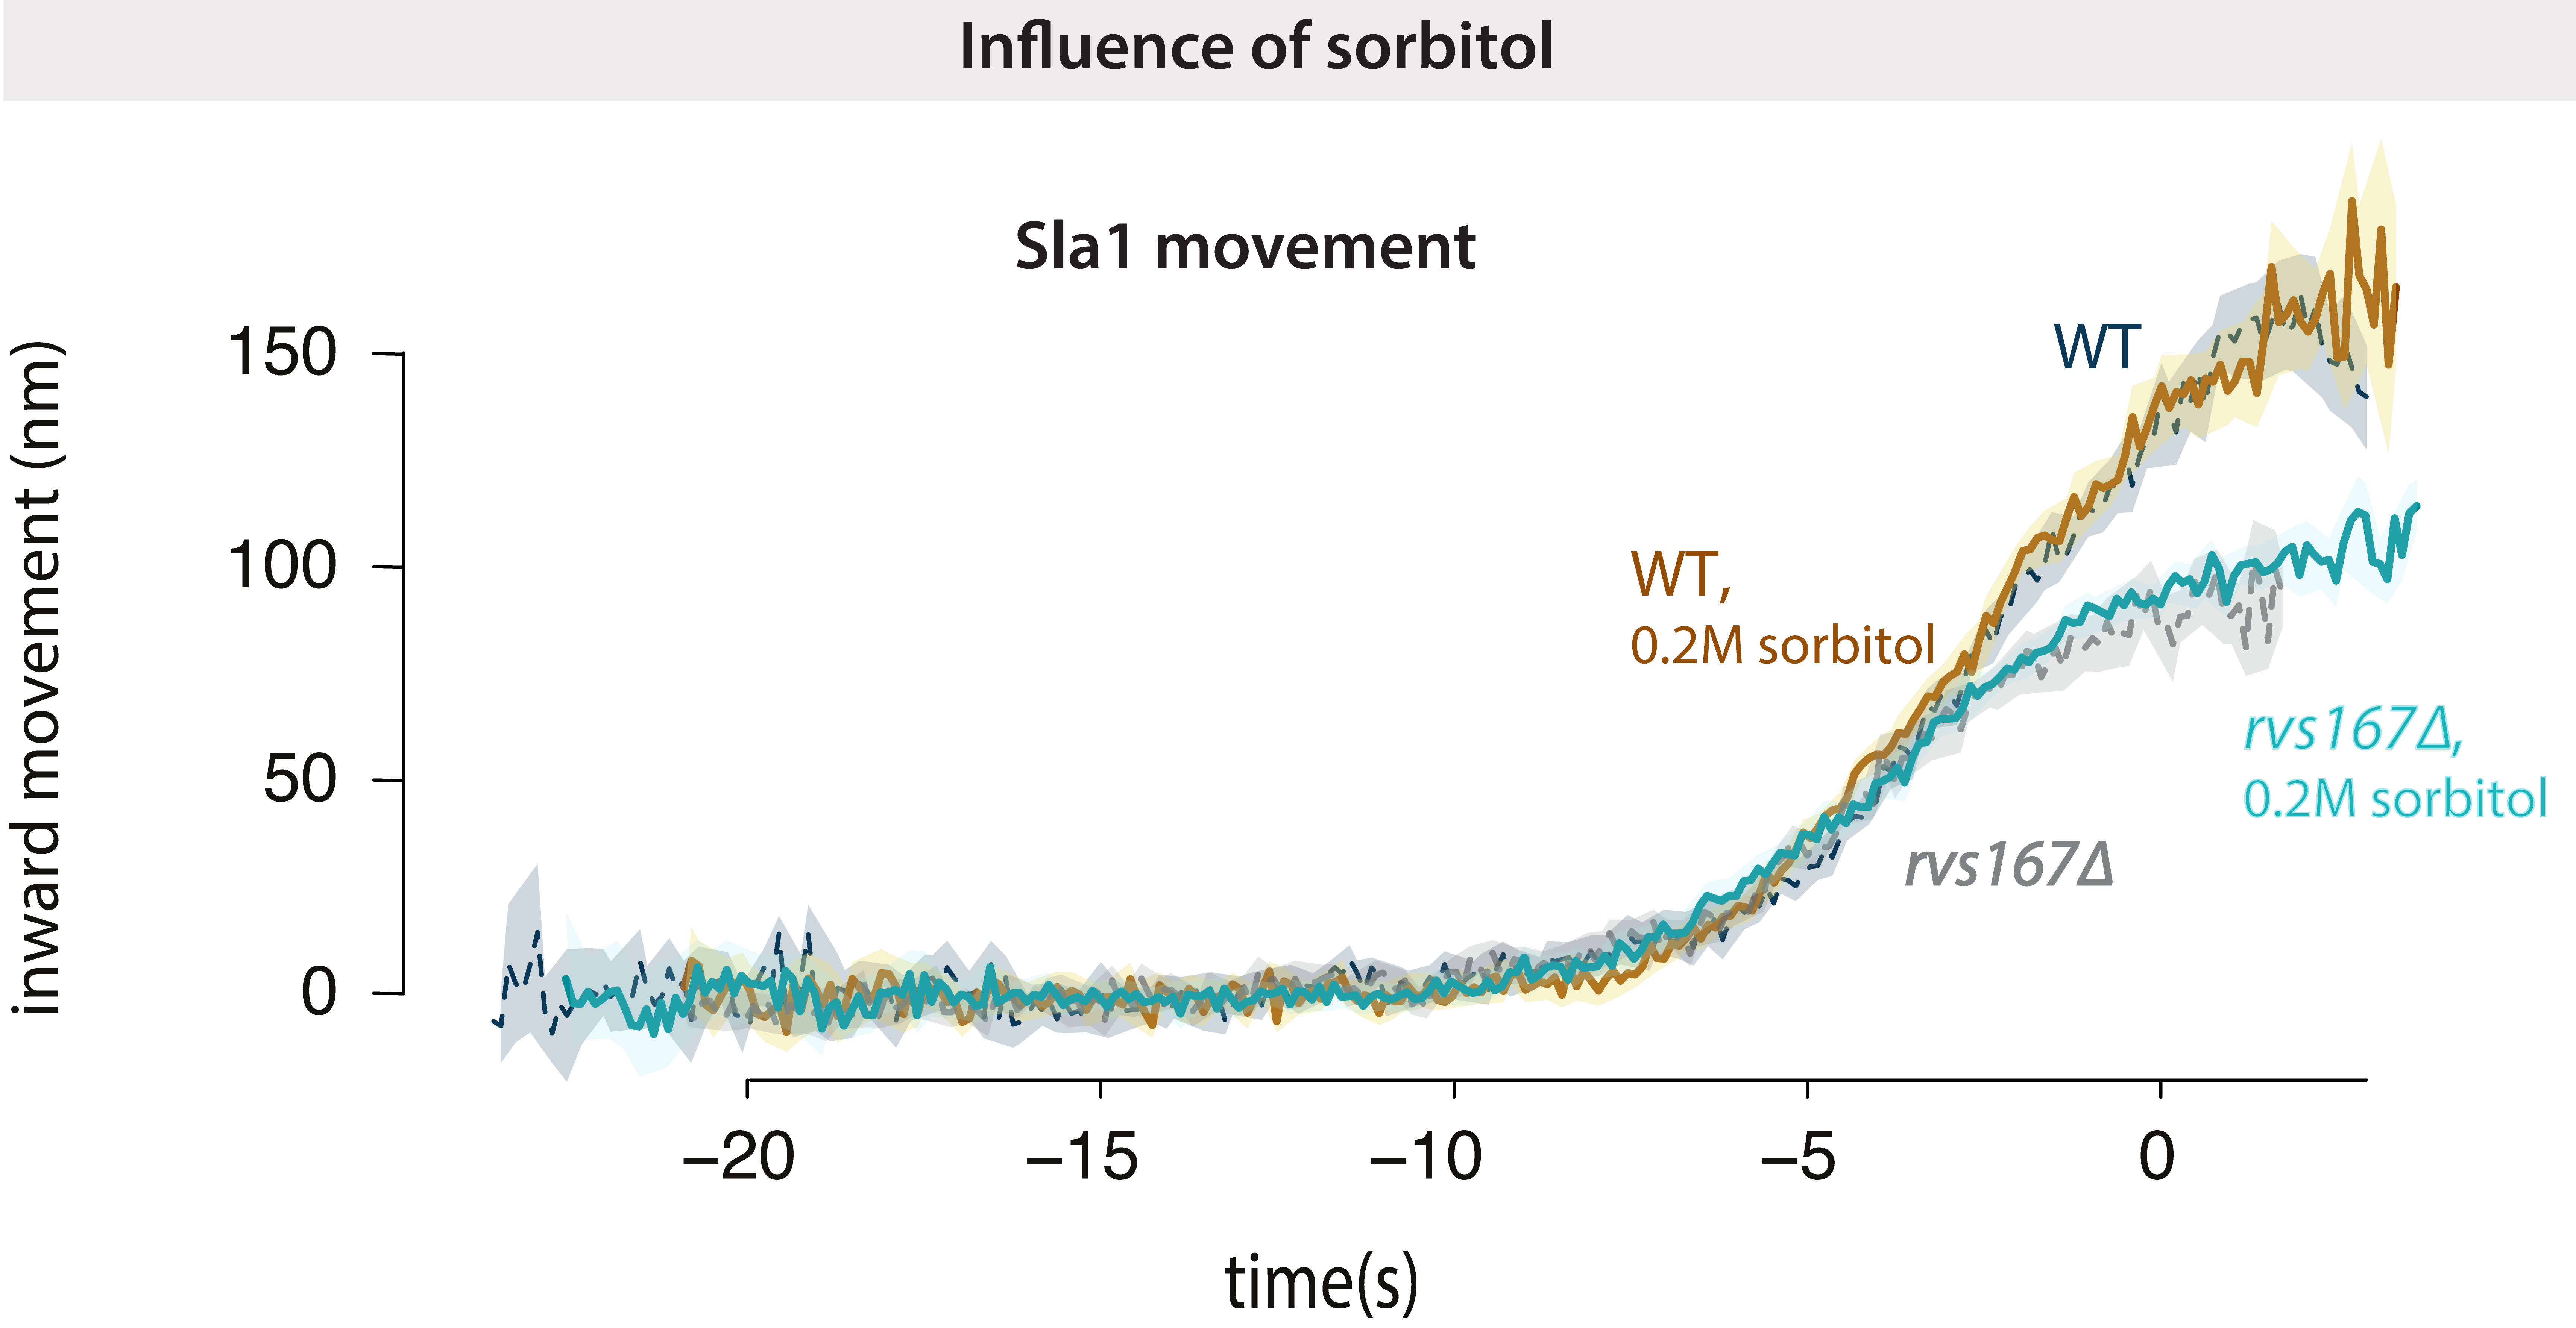
\includegraphics[width=10cm,height=10 cm,keepaspectratio]{figures/results_final/sorbitol2}
	\end{figure}

\newpage
\begin{table}[H]
	\centering
	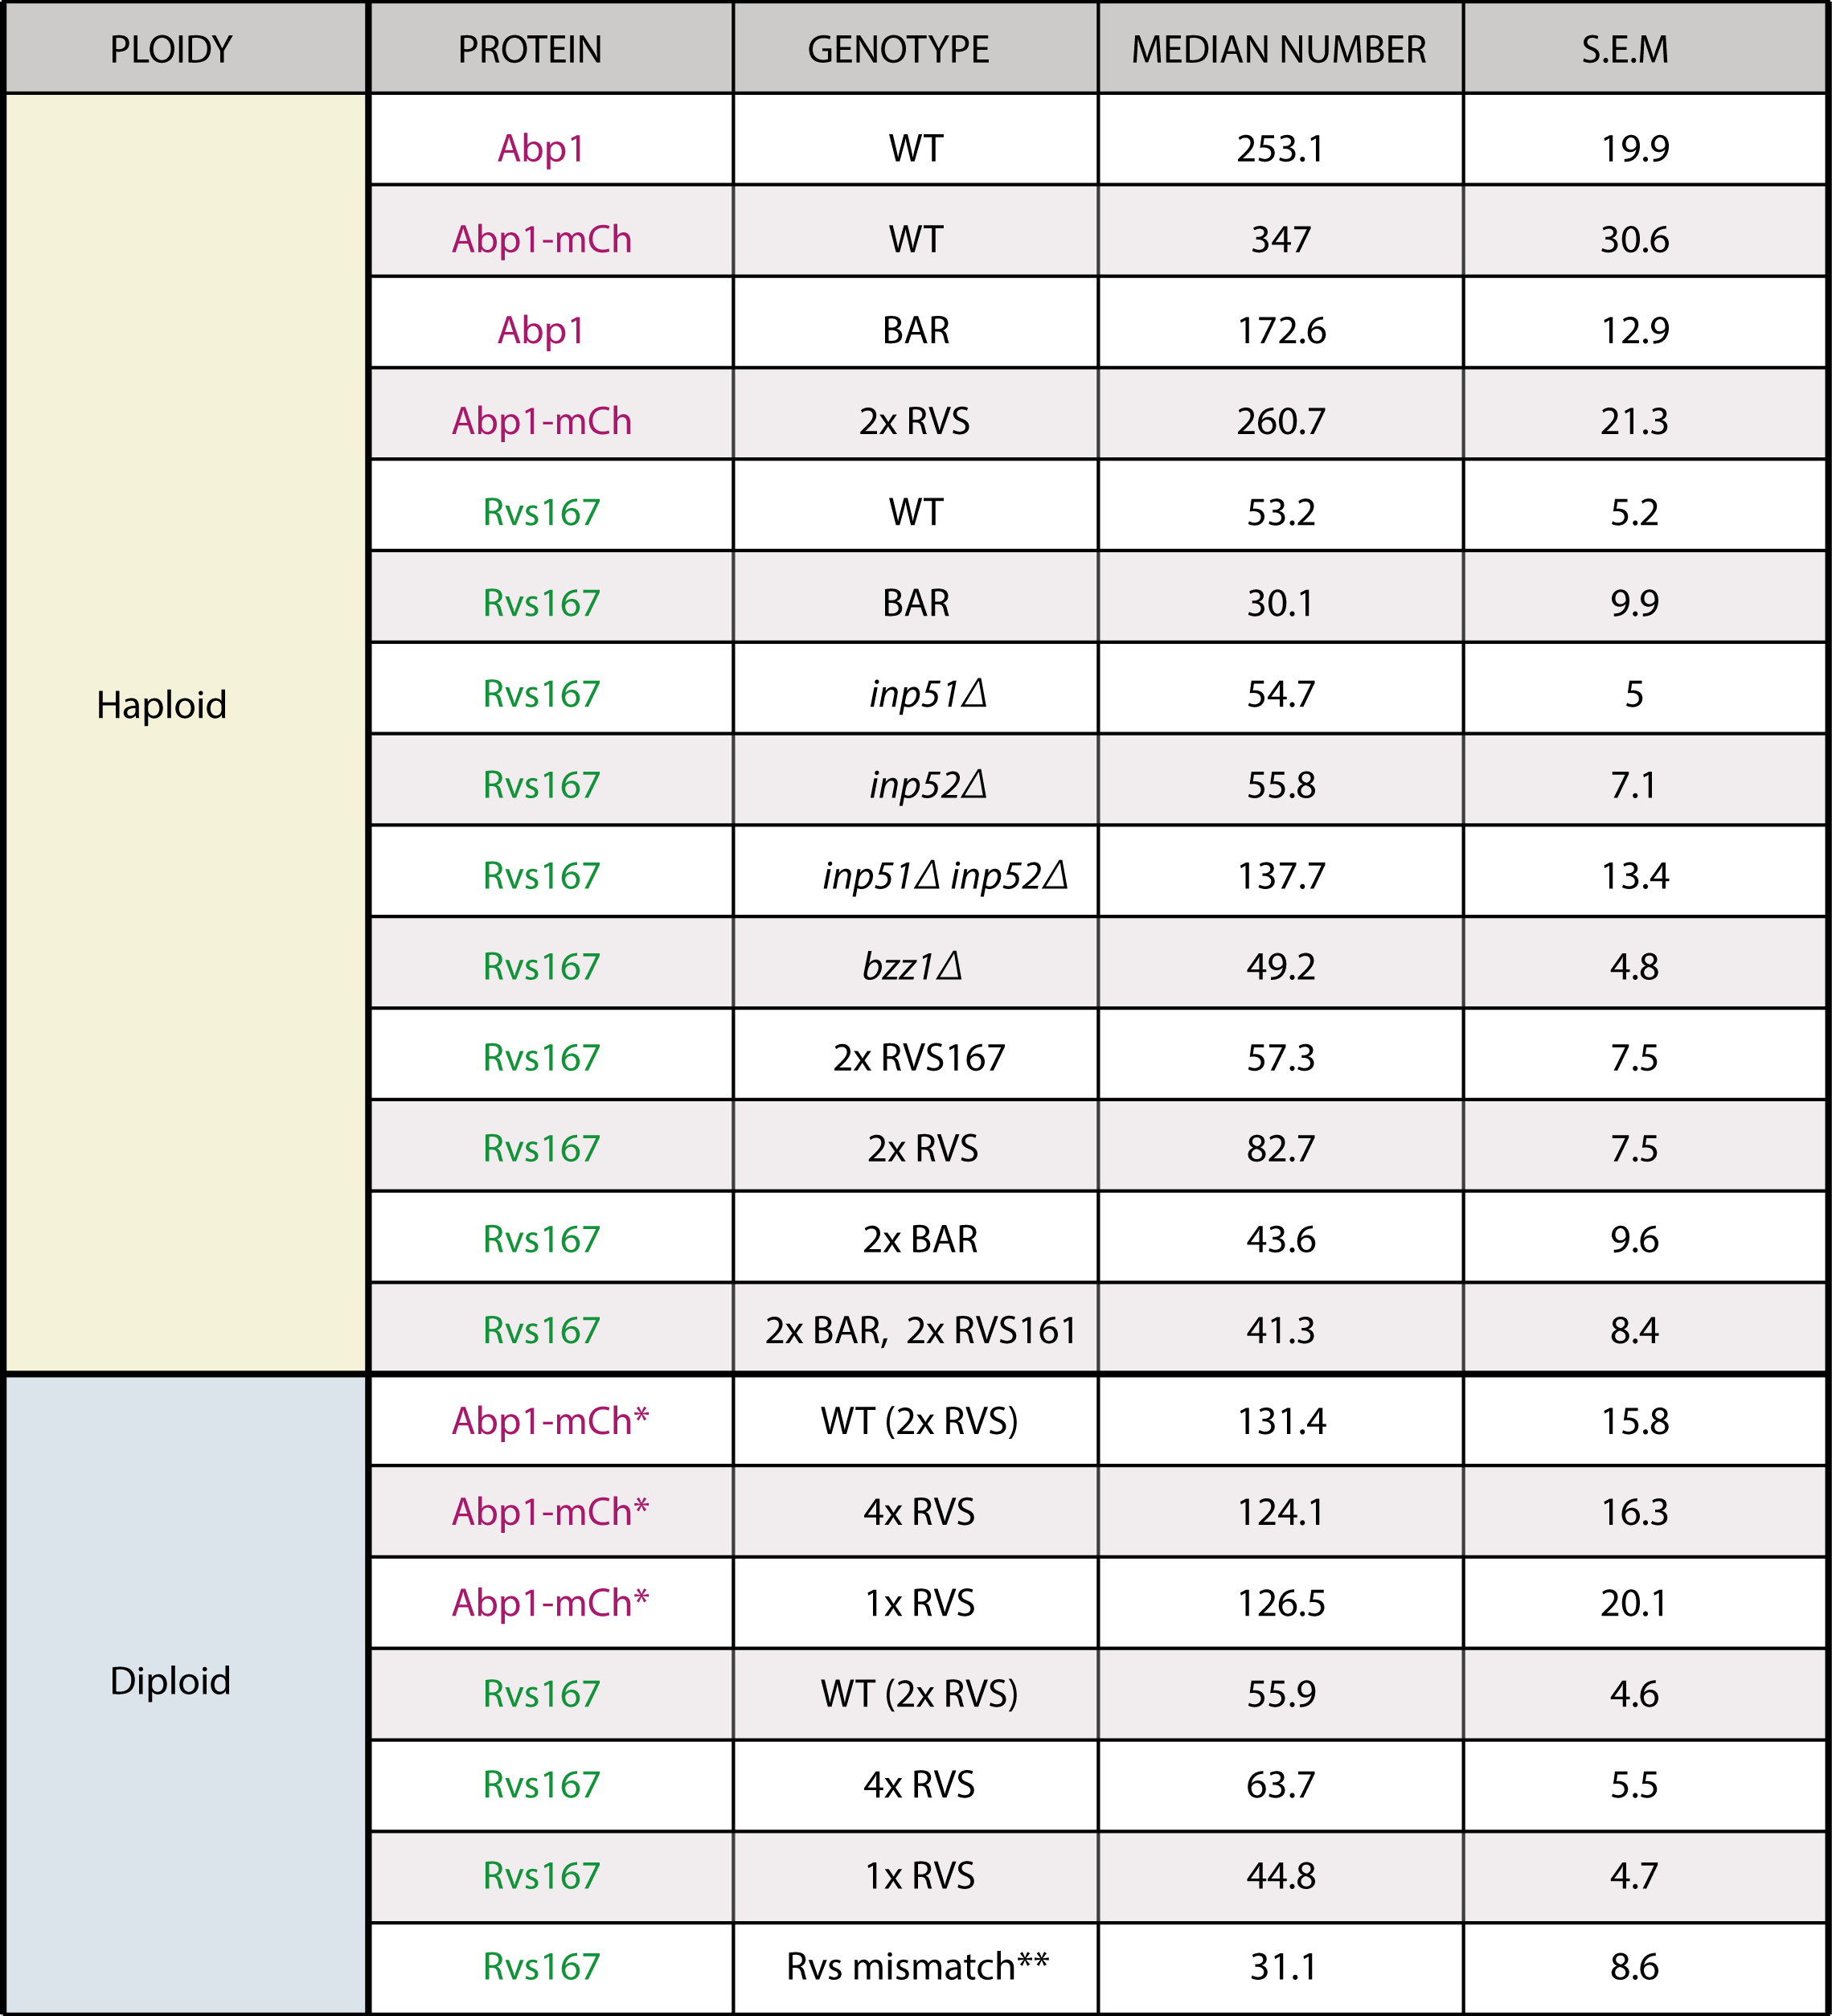
\includegraphics[width=16cm,height=25cm,keepaspectratio]{figures/results_final/table_numbers}
	%	\caption[Median molecule numbers]
\end{table}

